\documentclass{article}
\usepackage[UTF8]{ctex}
% Replace `letterpaper' with`a4paper' for UK/EU standard size
\usepackage[a4paper,top=2cm,bottom=2cm,left=3cm,right=3cm,marginparwidth=1.75cm]{geometry}

% Useful packages
\usepackage{amsmath}
\usepackage{mathrsfs,amsmath}
\usepackage{graphicx}
\usepackage[colorlinks=true, allcolors=blue]{hyperref}
\usepackage{graphicx} %插入图片的宏包
\usepackage{float} %设置图片浮动位置的宏包
\usepackage{subfigure} %插入多图时用子图显示的宏包
\usepackage{parskip}
\usepackage{indentfirst} 
\setlength{\parindent}{2em}
\usepackage{hyperref}  
\usepackage{tikz}
\allowdisplaybreaks
\usepackage{multirow}
\usepackage{amsmath}
\usepackage{amsfonts,amssymb} 
\usepackage{xcolor} % 用于显示颜色
\usepackage{listings} % 用于插入代码
\lstset{
	basicstyle          =   \sffamily,          % 基本代码风格
	keywordstyle        =   \bfseries,          % 关键字风格
	commentstyle        =   \rmfamily\itshape,  % 注释的风格,斜体
	stringstyle         =   \ttfamily,  % 字符串风格
	flexiblecolumns,                % 别问为什么,加上这个
	numbers             =   left,   % 行号的位置在左边
	showspaces          =   false,  % 是否显示空格,显示了有点乱,所以不现实了
	numberstyle         =   \zihao{-5}\ttfamily,    % 行号的样式,小五号,tt等宽字体
	showstringspaces    =   false,
	captionpos          =   t,      % 这段代码的名字所呈现的位置,t指的是top上面
	frame               =   lrtb,   % 显示边框
}

\lstdefinestyle{Python}{
	language        =   Python, % 语言选Python
	basicstyle      =   \zihao{-5}\ttfamily,
	numberstyle     =   \zihao{-5}\ttfamily,
	keywordstyle    =   \color{blue},
	keywordstyle    =   [2] \color{teal},
	stringstyle     =   \color{magenta},
	commentstyle    =   \color{red}\ttfamily,
	breaklines      =   true,   % 自动换行,建议不要写太长的行
	columns         =   fixed,  % 如果不加这一句,字间距就不固定,很丑,必须加
	basewidth       =   0.5em,
}

\title{数据结构Project-1报告:红黑树与B树 }
\author{林子开 21307110161}
\begin{document}
	\maketitle

\paragraph{摘要}
本文简要介绍了本次Project的整体项目架构,详细阐述了二叉搜索树(红黑树的父类)、红黑树
以及B树的代码实现与提供的基本操作方法。基于助教提供的测试样例,对红黑树和不同$t$值的B树
在5种操作上进行了耗时的对比与分析,并揭示出性能的差异。然后介绍了GUI界面的功能和防错检查机制。
最后简要阐述了在单词排列顺序上进行的创新改进。

	\tableofcontents

\section{文件简介与项目结构说明}
在codes文件夹下包含以下文件:
\begin{figure}[H]
	\centering
	{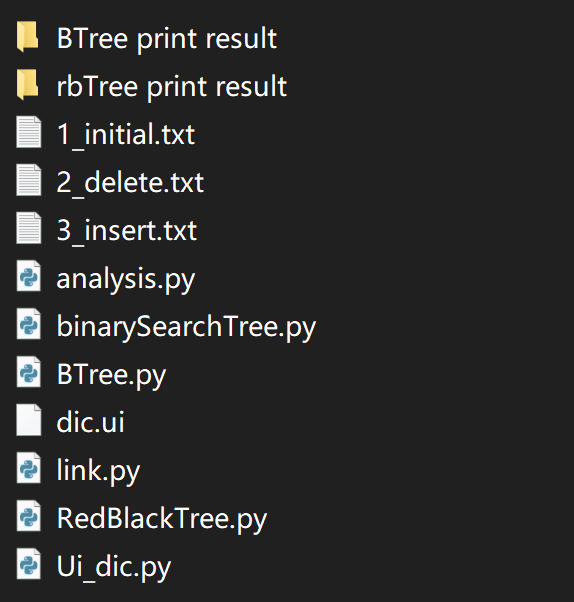
\includegraphics[width=0.4\textwidth]{image//文件说明.png}} 
	\caption{codes文件夹内的文件展示}
\end{figure}

codes文件夹里的文件简介:
\begin{itemize}
\item binarySearchTree.py文件中定义了二叉搜索树的节点node类与二叉树tree类,并提供了二叉树的基本操作。
\item RedBlackTree.py文件继承了binarySearchTree.py文件中的node与tree类,构建了红黑树的带颜色节点,
并实现了红黑树,该文件提供红黑树的增删改查操作,并能自动维护红黑树。
\item BTree.py文件中定义了B树的节点node类与BTree类,提供B树的增删改查等操作,并自动维护B树。
\item analysis.py文件则对红黑树与二叉树进行了五种操作的耗时测试,用于分析二者的优良性质。
\item dic.ui和Ui$\_$dic.py是用于构建GUI的文件,里面包含了的GUI的界面信息。(由于我不是软件学院的,
之前没有接触过UI方面的知识,是马上现学的,在这方面如有表述不清之处,还请助教谅解!)
\item link.py文件则用于连接GUI和数据结构,可以生成友好的交互界面,并提供基本的防错检查机制
(GUI的介绍详后)。
\item 1$\_$initial.txt,2$\_$delete.txt,3$\_$insert.txt 三个文件则是助教提供的用于测试的文件,
其中规定了要进行的操作,以及测试单词。
\item rbTree print result和BTree print result文件夹则分别保存了在红黑树和B树上根据
1$\_$initial.txt,2$\_$delete.txt,3$\_$insert.txt  三个文件进行操作后的结果。
其中,对红黑树的操作结果的记录文件命名格式为"rbt$\_$fileName.txt",其中fileName是上述三个助教提供的测试文件的文件名。
B树的操作结果的记录文件命名格式为"bt$\_$t=?$\_$fileName.txt",其中"?" 表示B树的t值,分别为5,10,15,20,25,
fileName意思同上。
\end{itemize}

这些文件的结构关系为:
\begin{figure}[H]
	\centering
	{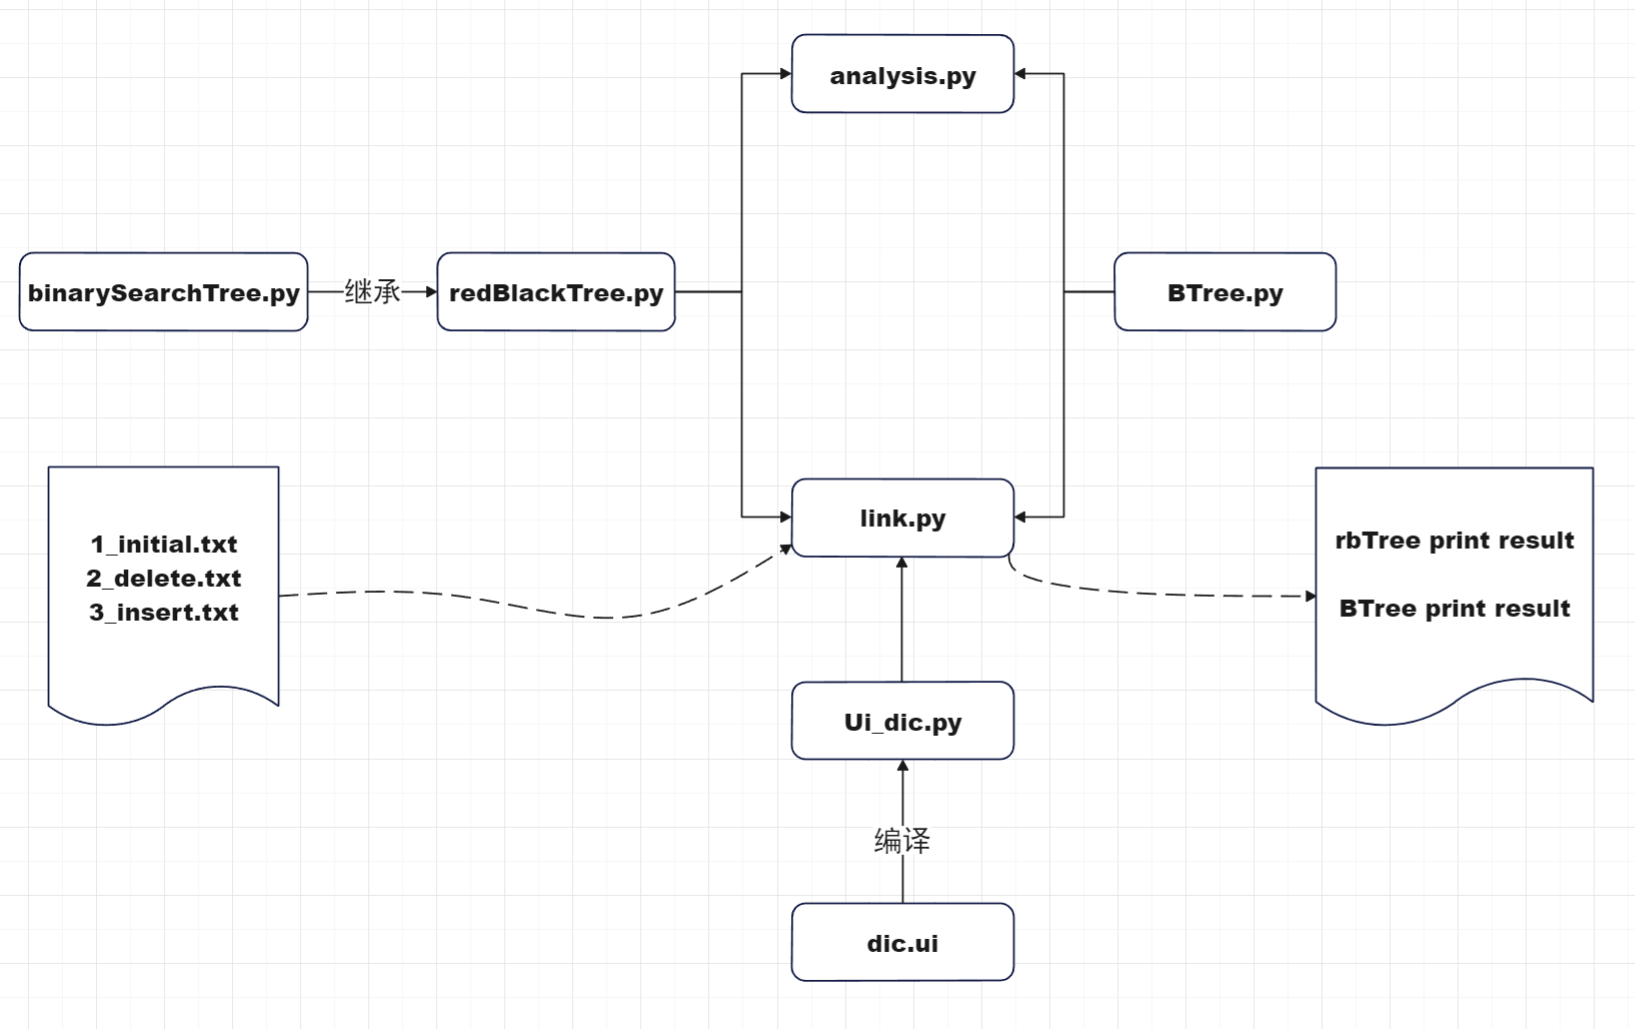
\includegraphics[width=0.8\textwidth]{image//项目结构.png}} 
	\caption{项目结构示意图}
\end{figure}


\section{binarySearchTree.py文件的主要功能介绍}
binarySearchTree.py文件实现了二叉搜索树。对于一棵二叉搜索树而言,其左子树的所有节点都小于父节点,
而右子树的所有节点都大于父节点。(关于英文单词的大小顺序说明,详后。)

该文件提供了关于二叉树的基本功能,包括增加一个子节点(put方法),删除一个子节点(delete方法),
查找一个子节点(get方法),中序遍历(inorder方法),先序遍历(preorder方法),向左旋转(left-rotation方法),
向右旋转(right-rotation方法),寻找后继节点(findSuccessor方法),寻找前驱节点(findPredecessor方法),
以及按范围搜索(rangeSearch方法)。其中,left-rotation与right-rotation方法是为红黑树做的准备。
由于左旋和右旋操作不涉及节点的颜色,因此将这两个方法定义在二叉搜索树(父类)上更为合适。

对于rangeSearch方法,如果两个边界词本身不是词典里已有的单词,或者本身就不是合法单词,
这里对返回的结果进行说明。例如,单词表内的单词按字典顺序为abuse, apple, bike, book, cat, catch. 
如果按照从"ab"开始,"ca"结束进行查询。那么,返回的单词,相当于把"ab"和"ca"先\textbf{“假装插入”}字典,
即,\underline{\textbf{ab}}, abuse, apple, bike, book, \underline{\textbf{ca}}, cat, catch. 
然后,返回这两个边界词中间的部分,也就是abuse, apple, bike, book 这四个单词。
如果边界词是词典里的单词,则返回的结果将包含边界词。rangeSearch的实现是通过调用findSuccessor方法
(复杂度为$\mathcal{O} (\log(n))$)
不断寻找当前节点的后继节点来完成的,因此rangeSearch操作的复杂度上界为$\mathcal{O} (n\log(n))$,
其中$n$是词典中的单词量。


\section{RedBlackTree.py文件的主要功能介绍}
RedBlackTree.py文件实现了红黑树这一数据结构,提供了对红黑树的基本操作,并自动维护红黑树的结构性质。
该文件中继承了binarySearchTree.py里的节点和二叉搜索树两个类,并且对其部分函数进行了重构。

对于红黑树中的节点,与二叉搜索树中的节点相比,多出了color这一属性。对于红黑树类,
则根据教材提供的伪代码,重构了父类(二叉搜索树)的插入(put)与删除(delete)方法,
这两个方法能够自动维护红黑树的平衡性,并且在\textbf{插入(put)和删除(delete)前,
都会调用父类的查找(get)方法,自动检查是否已经存在单词},以防止错误。

此外,还添加了专用于红黑树的先序遍历(RB-preorder)方法,该方法能够同时返回
节点所在的层数(level),节点是左子节点还是右子节点(child,用0/1)表示,以及返回节点存储单词与颜色(color)。

\section{BTree.py文件的主要函数功能介绍}
BTree.py文件则实现了B树这一数据结构。B树的特点是,所有的子节点都是等高的,并且每个节点最少有$t-1$个单词,
最多有$2t-1$个单词。

BTree.py中定义了三个基本的类:word, node, BTree。其中,word表示一个单词,存储了单词的英文与中文。
node是B树的节点,而BTree则是B树。 BTree.py提供了操作B树的基本功能,包括增加(put方法),删除(delete方法),
查找(get方法),先序遍历(B-preorder方法),按范围查找(rangeSearch方法)等。这些方法能够自动维护B树的结构。
其中,\textbf{调用插入(put)和删除(delete)方法会先自动调用查找(get)方法,
先检查词典中是否已经存在该单词},以防止错误。

其中,B树的先序遍历(B-preorder方法)为:先遍历所在节点的所有单词,然后再依次递归地遍历子树。
下面以教材中的图为例进行说明:
\begin{figure}[H]
	\centering
	{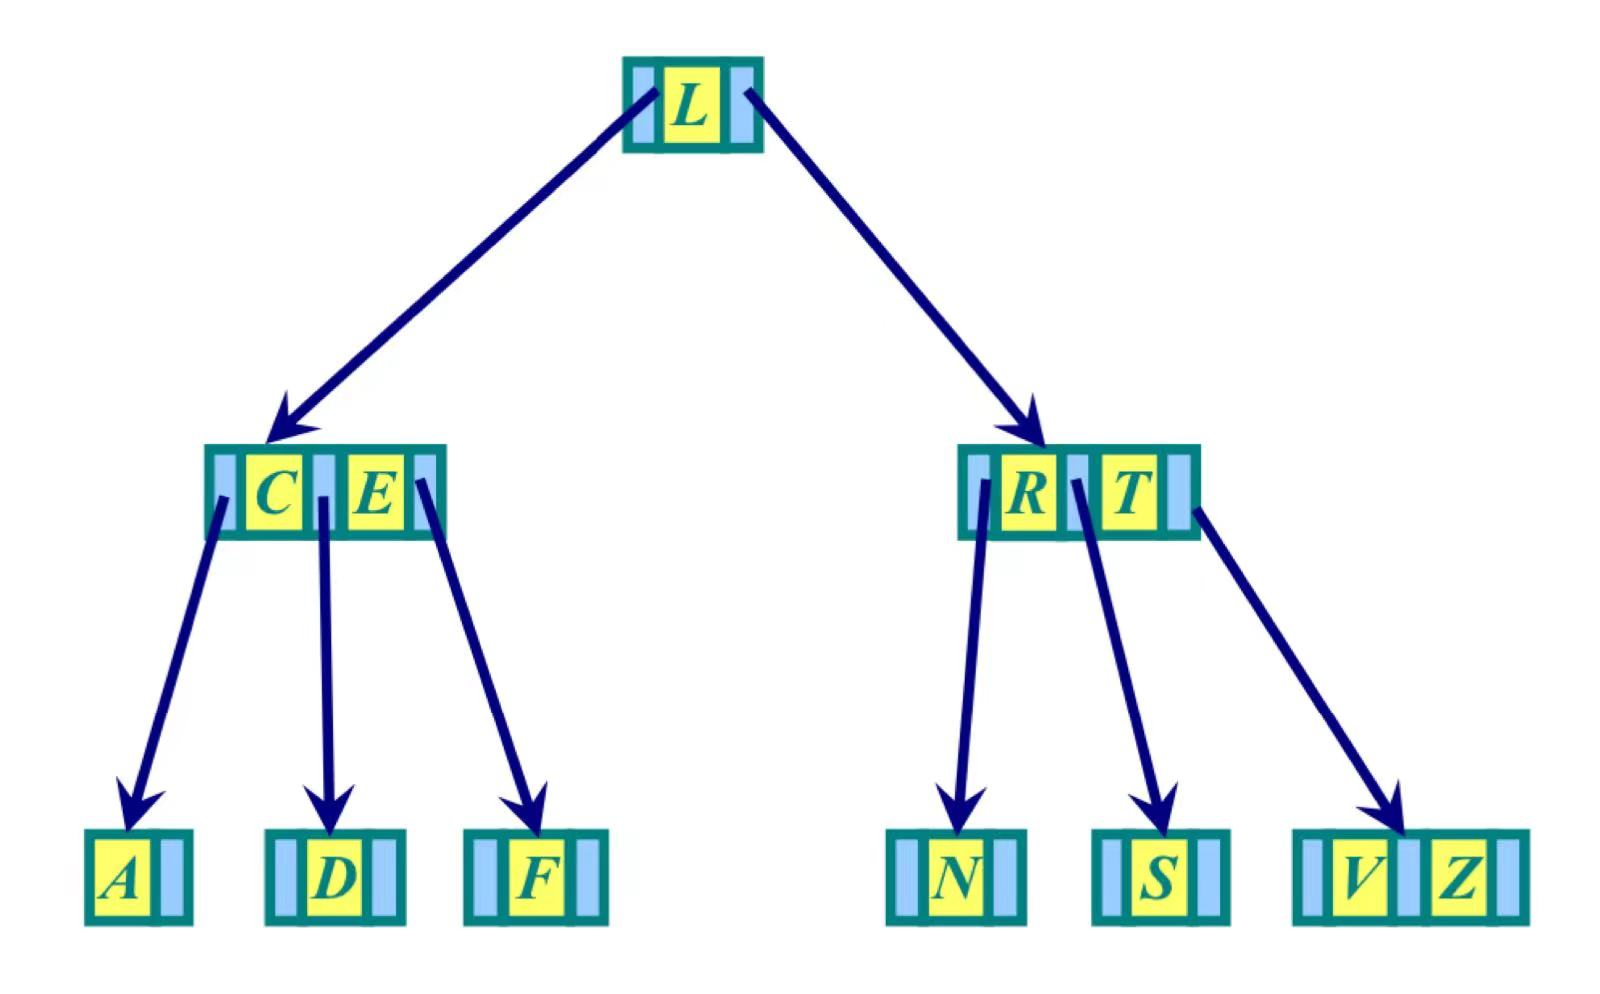
\includegraphics[width=0.5\textwidth]{image//先序遍历说明.jpg}}  
	\caption{B树示意图} \label{bt}
\end{figure}
如果对这颗B树进行先序遍历,则顺序应该为
\[L \rightarrow C \rightarrow E \rightarrow A \rightarrow D \rightarrow F \rightarrow  R \rightarrow  T \rightarrow N \rightarrow S \rightarrow V \rightarrow Z \]

除了返回单词,B-preorder方法也会反映当前节点所在的层数(level),
以及当前节点是父节点的第几个子节点(根节点默认为0)。

关于B树的findSuccessor方法,这里也进行说明。由于B树中的节点没有定义parent属性
(考虑到B树的适用场合,不应该定义节点的parent属性),这导致无法使用二叉搜索树的findSuccessor方法。
于是,我给出的findSuccessor方案是:
\begin{enumerate}
	\item 如果当前单词所在节点不是叶子节点,则返回“右子树”的最小节点。这里的“右”子树
			指的是和当前单词紧邻的右侧子树。例如,在图\ref{bt}中,
			例如要寻找R的后继者,由于R所在的节点不是叶子节点,则在紧邻R的右子树(即包含S的子树)中
			寻找最小单词(也就是S)作为后继者。
	\item 如果当前单词所在节点是叶子节点,但当前单词不是该叶子节点的最大单词,则返回其右侧的单词。
			例如在图\ref{bt}中,V所在的节点是叶子节点,但并不是该节点的最大单词,因此返回Z作为其后继。
	\item 如果当前单词所在节点是叶子节点,并且当前单词是该叶子节点的最大单词,则从root节点出发一路走到当前节点,
			并记录最后一次作为“左子节点”时刻的父节点。例如,在图\ref{bt}中,A是当前节点最大的单词,
			因此,则重新从root节点L出发,先向左走到C节点(此时C是L的“左”子节点,记录下L),然后,
			再从C出发向左走到A节点(此时A是C的“左”子节点,记录下C),由于已经找到A,则结束循环,此时
			最后一次记录下的C节点就是A的后继。
\end{enumerate}

由以上分析可知,B树的findSuccessor方法的复杂度上界为$\mathcal{O} (\log(n))$,而B树的rangeSearch方法
也同样是不断调用findSuccessor方法实现的,因此,我设计的对于B树的rangeSearch方法的复杂度也同样为$\mathcal{O} (n\log(n))$,
其中$n$是词典中的单词量。

\section{操作时间分析}
下面,我们分别对红黑树,以及具有不同$t$值的B树进行以下五种操作,分析他们的耗时。
\begin{enumerate}
	\item 按照1$\_$initial.txt文件的要求,插入单词,对词典进行初始化;
	\item 按照2$\_$delete.txt文件的要求,删除单词,在删除单词时候,delete方法会自动检查单词是否存在;
	\item 按照3$\_$insert.txt文件的要求,插入单词,在插入单词时,put方法会自动检查单词是否已经存在;
	\item 调用get方法,查询一个单词;
	\item 调用rangeSearch方法,查询某个范围内的单词。
\end{enumerate}

在上述的5个操作中,根据本次Project要求,在前三个步骤中,每进行100个单词的操作,
就要记录一次对这100个单词操作的耗时。由于1$\_$initial.txt中有3300个单词,则要记录33次耗时。
而2$\_$delete.txt与3$\_$insert.txt都各只有100个单词,因此只要各自记录一次时间。

由于查询单词的时间比较短,因此,对于第4和第5个操作,需要多次操作然后取平均值,得到更为准确的测量。
在本次实验中,我们对"concisely"这个单词进行1000次查找,然后计算平均用时。
此外,对从"afr"到"cu"范围内的单词进行100次查找,然后计算平均用时。以下是实验的结果。


\subsection{红黑树操作时间分析}
对红黑树进行第一项操作时,记录的耗时结果为:
0.00200057, 0.004001379, 0.004000664, 0.005000591,
0.004000664, 0.004001141, 0.006001711, 
0.006000996, 0.004001141, 0.006001711, 
0.00500083, 0.005001068, 0.006000519, 0.005002499, 
0.005004168, 0.005001545, 0.005002022, 0.00500083, 
0.006000996, 0.005001783, 0.005001307, 
0.006000519, 0.00500083, 0.005001783, 0.006000757, 
0.005001307, 0.006001234, 0.006001711, 
0.006000757, 0.005001545, 0.0070014, 0.006002188, 
0.006000042

由于以上耗时结果比较冗杂,于是做出折线图如下:
\begin{figure}[H]
	\centering
	{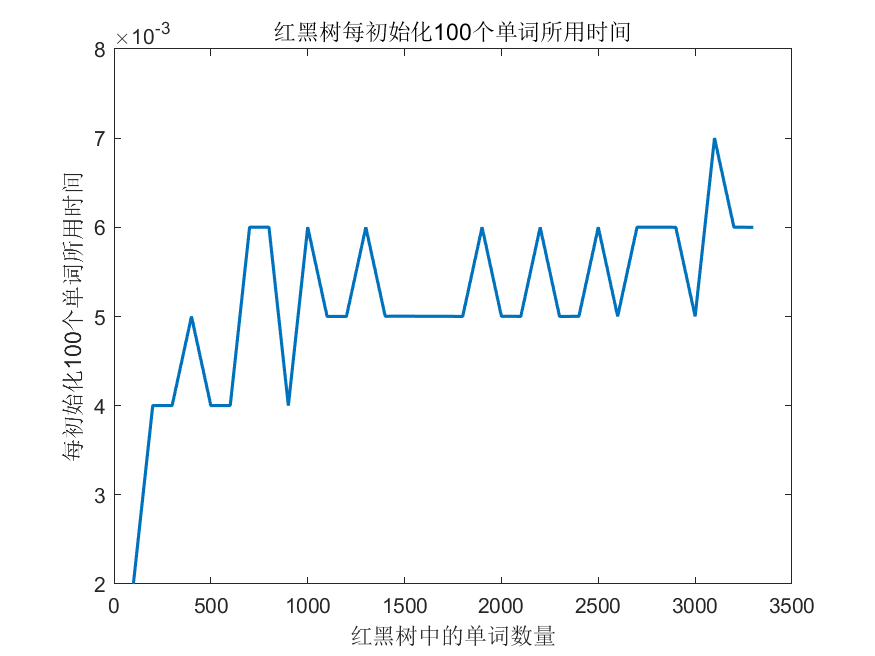
\includegraphics[width=0.85\textwidth]{时间图像绘制/rbTree_init.png}} 
	\caption{红黑树初始化的用时}
\end{figure}

可以看出,随着单词数量的增加,红黑树的插入时间呈现\textbf{对数增长},这与理论结果是吻合的。

将剩余所有操作的消耗时间列表如下:

\begin{table}[H]
	\centering
	\caption{红黑树的操作用时}
	\begin{tabular}{ll}
		\hline
	\textbf{对红黑树的操作}           & \textbf{耗时}           \\
	\hline
	初始化3300个单词总耗时     & 0.0060000420 \\
	删除100个单词          & 0.0030002594 \\
	插入100个单词          & 0.0040023327 \\
	查询单词"concisely"   & 0.0000150030 \\
	查询"afr"到"cu"范围内单词 & 0.0036185813 \\ 
	\hline
	\end{tabular}
	\end{table}


\subsection{B树操作时间分析}
我分别对$t=5, 10, 15, 20, 25$几种情况做了分析。

对于初始化情况,由于数据比较冗杂,请在附录中查看原始数据。这里仅展示时间变化的曲线图如下:
\begin{figure}[H]
	\centering
	{\includegraphics[width=0.85\textwidth]{时间图像绘制/BTree_init.png}} 
	\caption{不同t值的B树初始化用时}
\end{figure}

在图中,随着B树种单词的数量增加,每插入100个单词的消耗时间也基本呈现对数增长的趋势。
其中有少量的耗时为0的时间点,可能是因为耗时太小,无法被python的time()函数所准确记录导致的。

比较具有不同$t$值的B值的初始化耗时,可以发现,在本次实验中,$t=5$的B树在初始化操作上,具有最好的时间性能。
这也说明了对B树而言,$t$值并非越大越好。

对具有不同$t$值的B树进行余下四项操作,将其耗时整理如下表:

\begin{table}[H]
	\centering
	\caption{不同t值的B树的操作时间}
		\begin{tabular}{lccccc}
		\hline
											  & \multicolumn{5}{c}{\textbf{t of B-tree}}                                                                                  \\
											  & \multicolumn{1}{l}{5} & \multicolumn{1}{l}{10} & \multicolumn{1}{l}{15} & \multicolumn{1}{l}{20} & \multicolumn{1}{l}{25} \\ \hline
		\textbf{operation}                    & \multicolumn{1}{l}{}  & \multicolumn{1}{l}{}   & \multicolumn{1}{l}{}   & \multicolumn{1}{l}{}   & \multicolumn{1}{l}{}   \\
		initial 3330 words                    & 0.0040006638          & 0.0049996376           & 0.0078995228           & 0.0070014000   		& 0.0080015659           \\
		delete 100 words                      & 0.0040006638          & 0.0050272942           & 0.0060012341           & 0.0082633495           & 0.0093033314           \\
		insert 100 words                      & 0.0057239532          & 0.0035190582           & 0.0070011616           & 0.0094175339           & 0.0093631744           \\
		search the word  "concisely"         & 0.0000143282          & 0.0000272236           & 0.0000351186           & 0.0000202103           & 0.0000702636           \\
		search words in range & 0.0094751883          & 0.0061630583           & 0.0052250123           & 0.0045470905           	& 0.0054226136           \\ \hline
		\end{tabular}
		\end{table}

	同时,将各操作的时间与$t$的关系绘图如下:

	\begin{figure}[H]
    \centering
    \subfigure[删除100个单词]
    {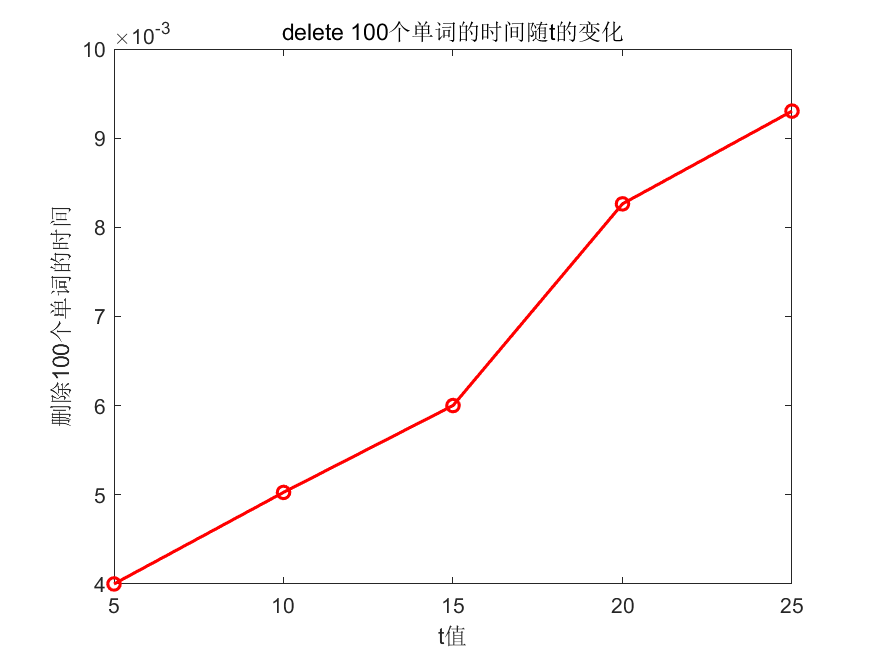
\includegraphics[width=0.49\textwidth]{时间图像绘制//Btree_delete100.png}}
    \,    
    \subfigure[插入100个单词]
    {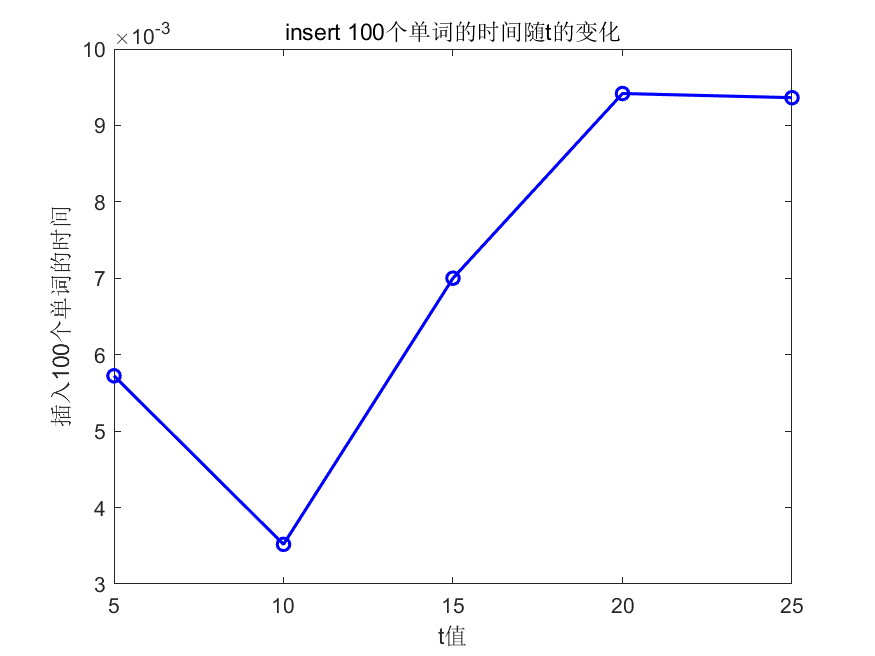
\includegraphics[width=0.49\textwidth]{时间图像绘制//Btree_insert100.png}}
    \,
    \subfigure[查询一个单词"concisely"]
    {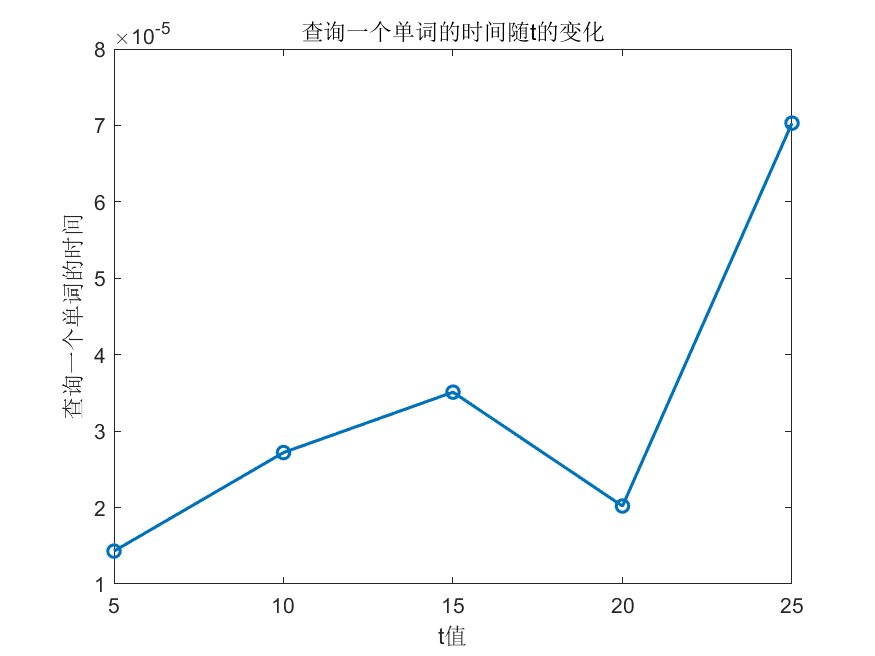
\includegraphics[width=0.49\textwidth]{时间图像绘制//Btree_search.png}}
    \,    
    \subfigure[查询"afr" 到 "cu" 范围内的单词]
    {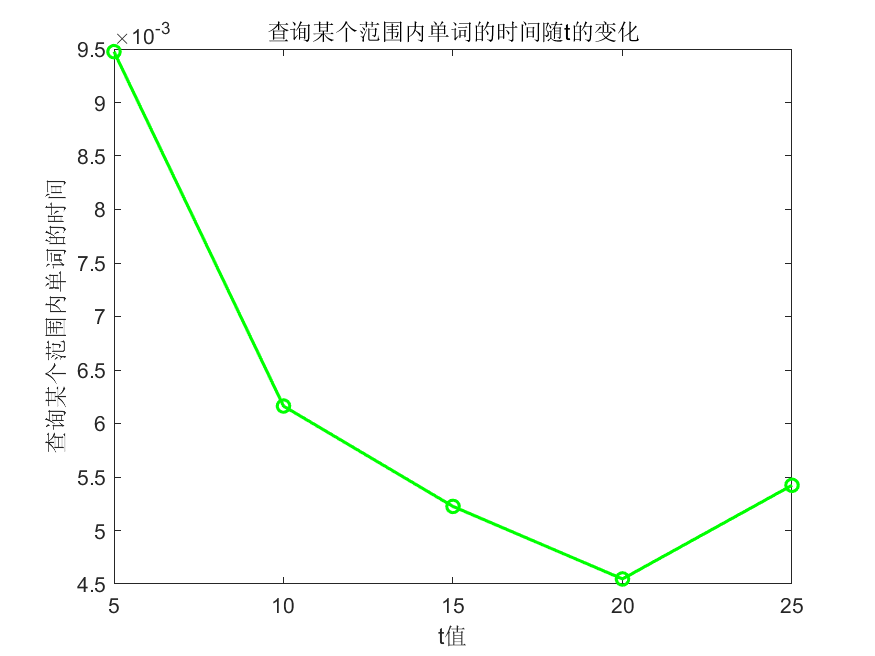
\includegraphics[width=0.49\textwidth]{时间图像绘制//Btree_rangeSearch.png}}
    \caption{local equalization with different patch sizes}
\end{figure}

从以上各图可以看出,对于删除操作而言,$t=5$时有最少的删除时间。对于插入操作而言,
$t=10$时有最少的插入时间。对于查询一个单词而言,$t=5$时有最少的查询时间。
而对于查询某个范围内的单词而言,$t=20$时有最少的查询时间。这说明,对于不同的B树上的操作,
最优的$t$是不同的,在实际设计中,应该根据现实场景,判断哪种操作最为频繁,进而选择适合于实际的$t$值。

除此之外,和红黑树相比,$t=5$时的B树的各项操作的时间开销与红黑树基本接近,
但是当$t\ge 10$的时候,B树的时间开销逐渐超过红黑树,性能逐渐变得比红黑树差。
这说明在每个节点的存储开销比较小时,使用红黑树或者$t$值较小的B树是比较合理的。

\section{GUI功能简介与防错机制}
本小节简要介绍GUI的各部分功能,以及我设计的一些防错检查机制。

\paragraph{启动GUI} 运行link.py文件,可以得到如下界面:

\begin{figure}[H]
	\centering
	{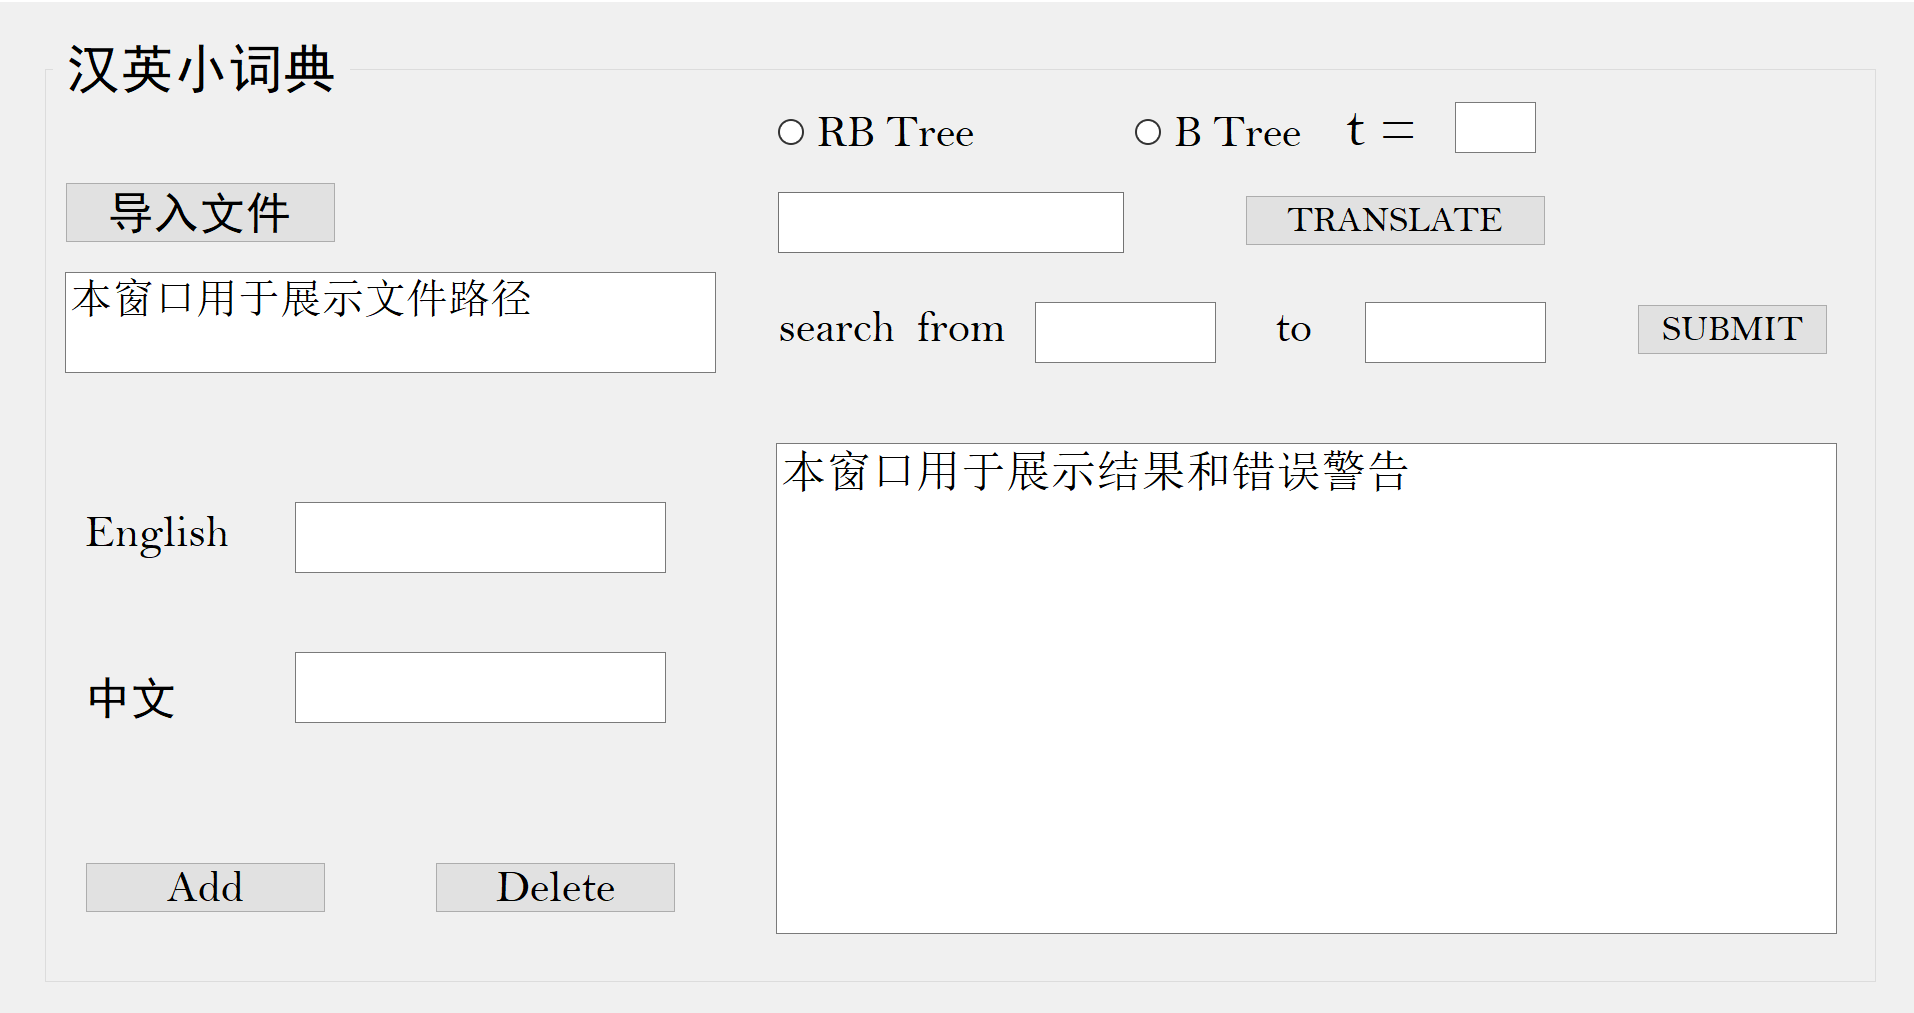
\includegraphics[width=0.5\textwidth]{GUI//启动界面.png}} 
	\caption{启动界面}
\end{figure}

界面左半部分提供了选择导入执行文件,以及插入、删除单词的功能。
界面的右半部分提供了选择数据结构类型(红黑树/B树),查询某个单词,以及按照范围查词的功能。
界面的右下角的空白区域用于展示查询结果、抛出错误警告等。


\paragraph{选择建立红黑树/B树}在界面的右上角,可以选择建立一棵红黑树,或者一棵B树。如果建立B树,还需要输入t值。
如果在没有选择建立何种类型的树的情况下,就点击其他按钮,则会抛出异常警告,如图\ref{tree.sub.1}所示。
对于B树,如果没有输入t值就建立B树,也同样会抛出警告,如图\ref{tree.sub.2}所示。
用户需要输入合适的t值($t\ge$2),否则同样也会抛出警告。
成功建立红黑树或者B树后,界面也会进行提示,如图\ref{tree.sub.3}所示。

\begin{figure}[H]
    \centering
    \subfigure[未建立树时点击其他按钮会报错] 
    {\label{tree.sub.1}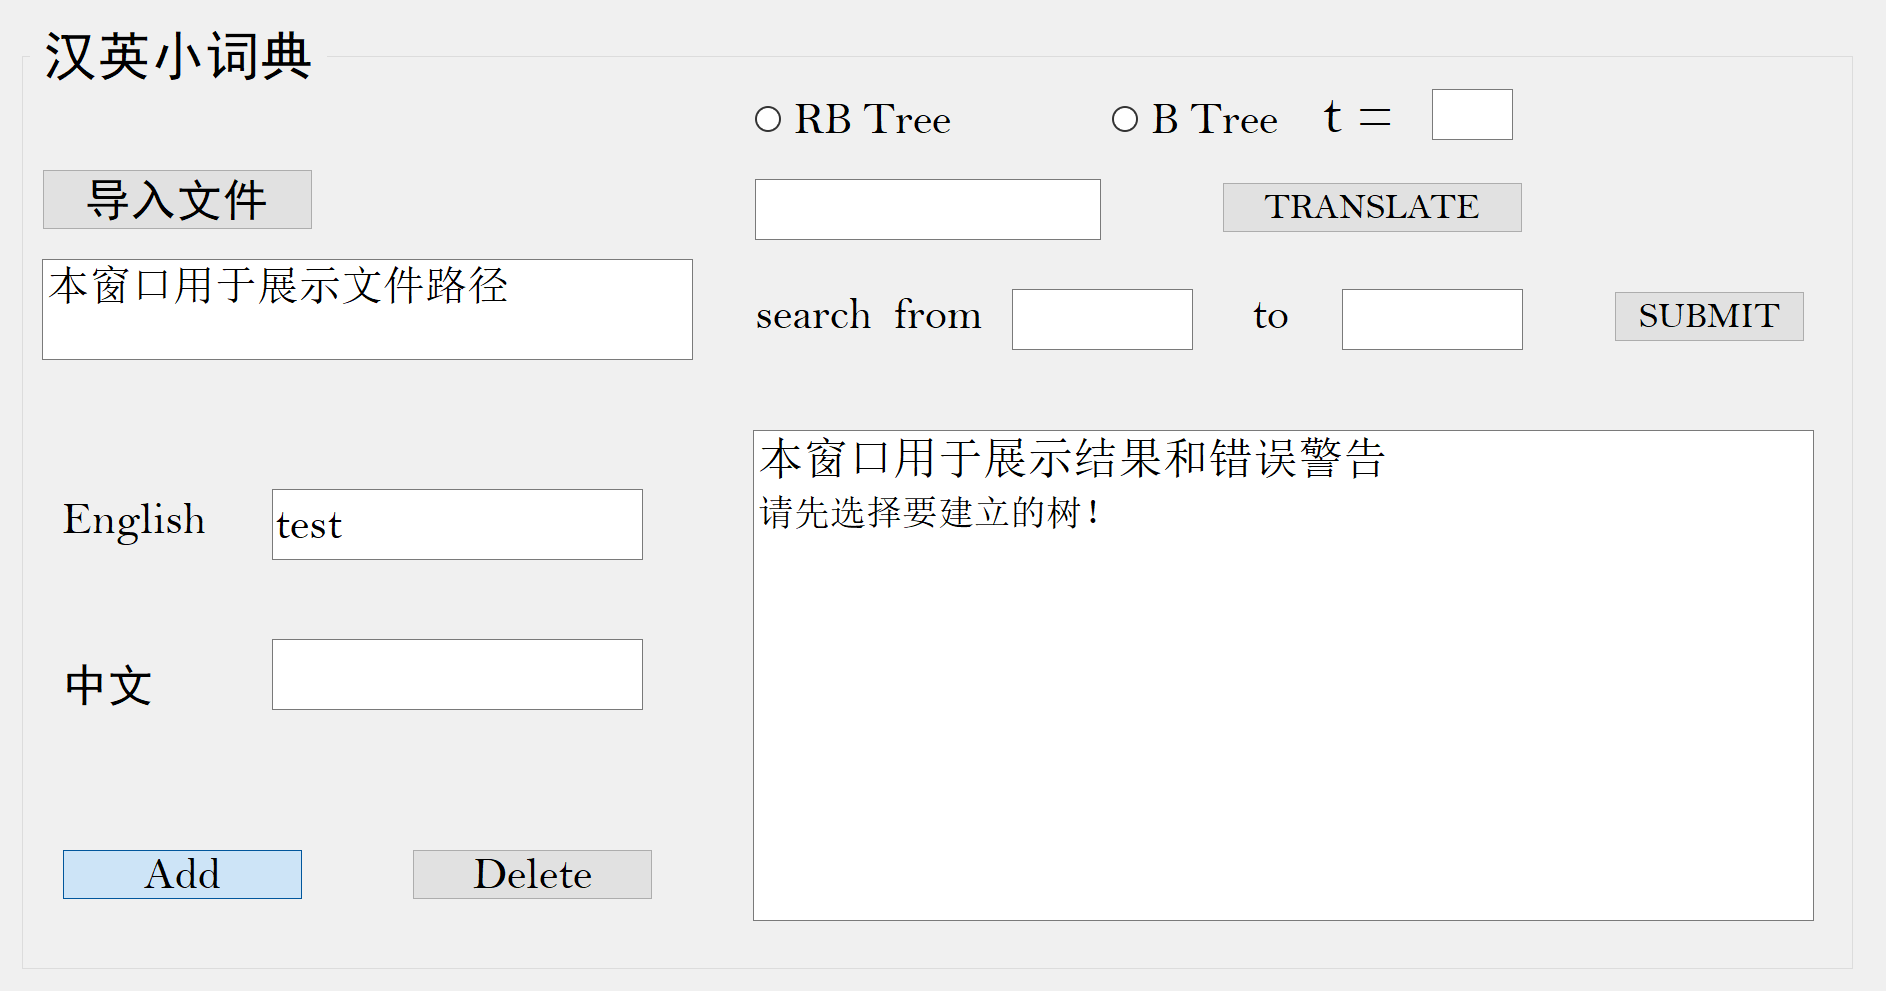
\includegraphics[width=0.3\textwidth]{GUI//先建树.png}}
    \,    
    \subfigure[未输入t值也会报错]
    {\label{tree.sub.2}\includegraphics[width=0.3\textwidth]{GUI//B树t.png}}
	\,
	\subfigure[成功建立树]
    {\label{tree.sub.3}\includegraphics[width=0.3\textwidth]{GUI//B树t-correct.png}}
	\caption{选择树的种类并建立树}
	\label{tree.main}
\end{figure}

在接下来的演示中,都以$t=5$的情况为例进行说明。

\paragraph{导入并执行测试文件}在界面的左上角有一个导入文件按钮,点击后会出现弹窗,可以选择要导入的文件,如图\ref{import.sub.1}所示。
在该按钮的下方有一个文本显示器,会显示出用户选择的执行文件的绝对路径,
在成功执行完对应文件之后,\textbf{会自动把当前的词典按照先序遍历的方式打印到对应的文件夹内}, 
同时,界面右下方会抛出对应的提示,如图\ref{import.sub.2}所示。

\begin{figure}[H]
    \centering
    \subfigure[点击导入文件按钮弹出对话框] 
    {\label{import.sub.1}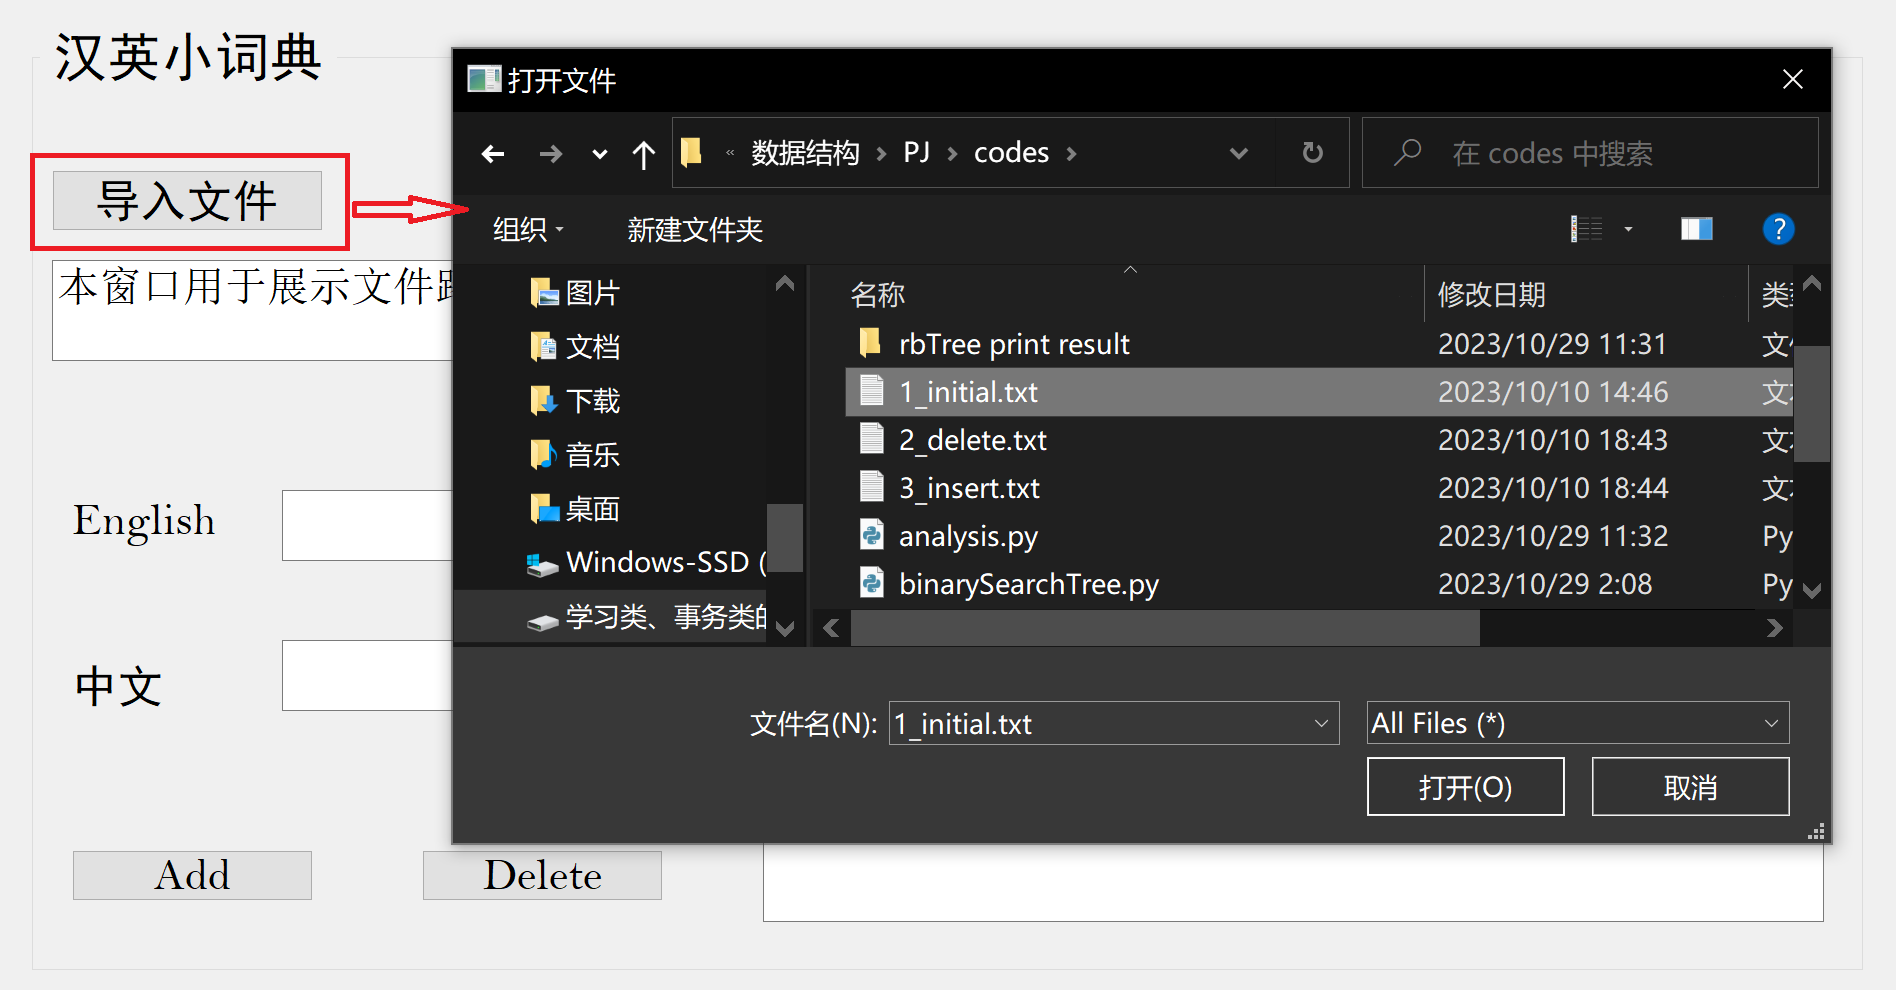
\includegraphics[width=0.45\textwidth]{GUI//导入文件.png}}
    \,    
    \subfigure[执行文件后会有提示]
    {\label{import.sub.2}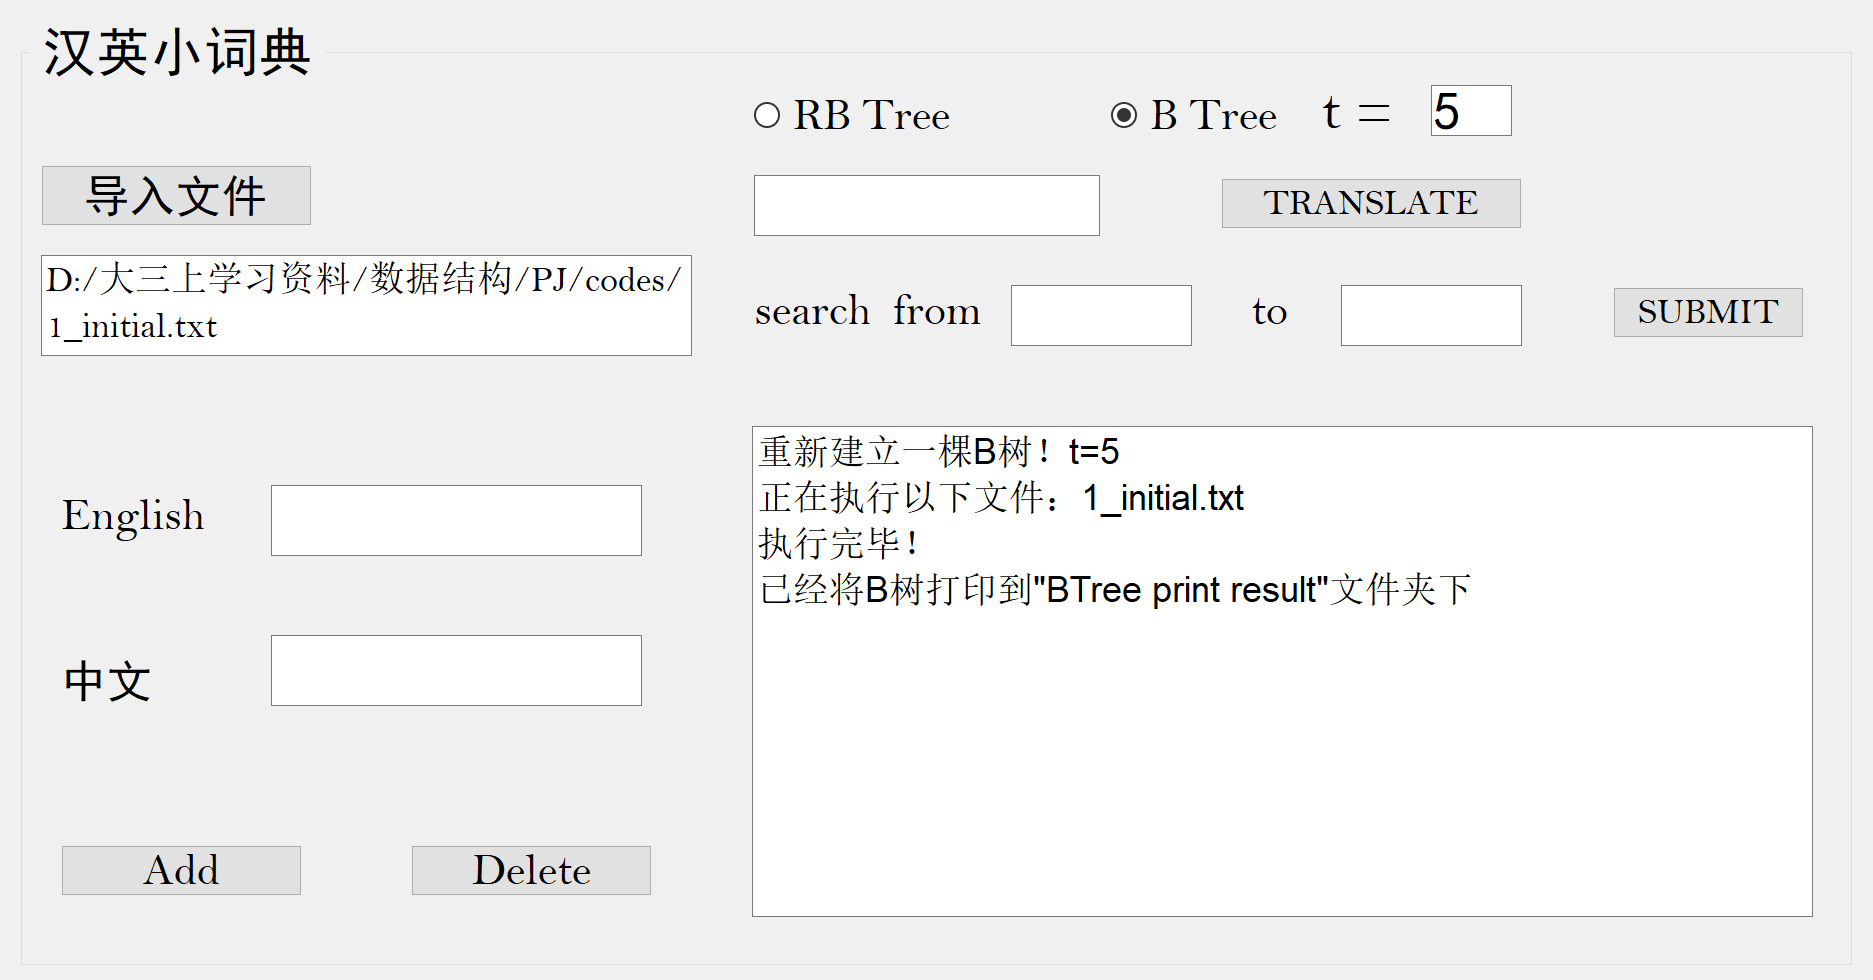
\includegraphics[width=0.45\textwidth]{GUI//执行文件.png}}
	\caption{选择导入文件}\label{import.main}
	
\end{figure}


\paragraph{添加新单词}在界面的左下方,有两个文本框,上方的文本框用于输入英文单词,
下方的文本框用于输入中文释义。点击"Add"按钮,如果词典中没有这个单词,则可以将单词添加到词典中,
如图\ref{add.sub.1}所示。如果词典中已经存在这个单词,则无法插入,并会抛出错误提示,
如图\ref{add.sub.2}所示。

\begin{figure}[H]
    \centering
    \subfigure[插入一个原本不存在的单词] 
    {\label{add.sub.1}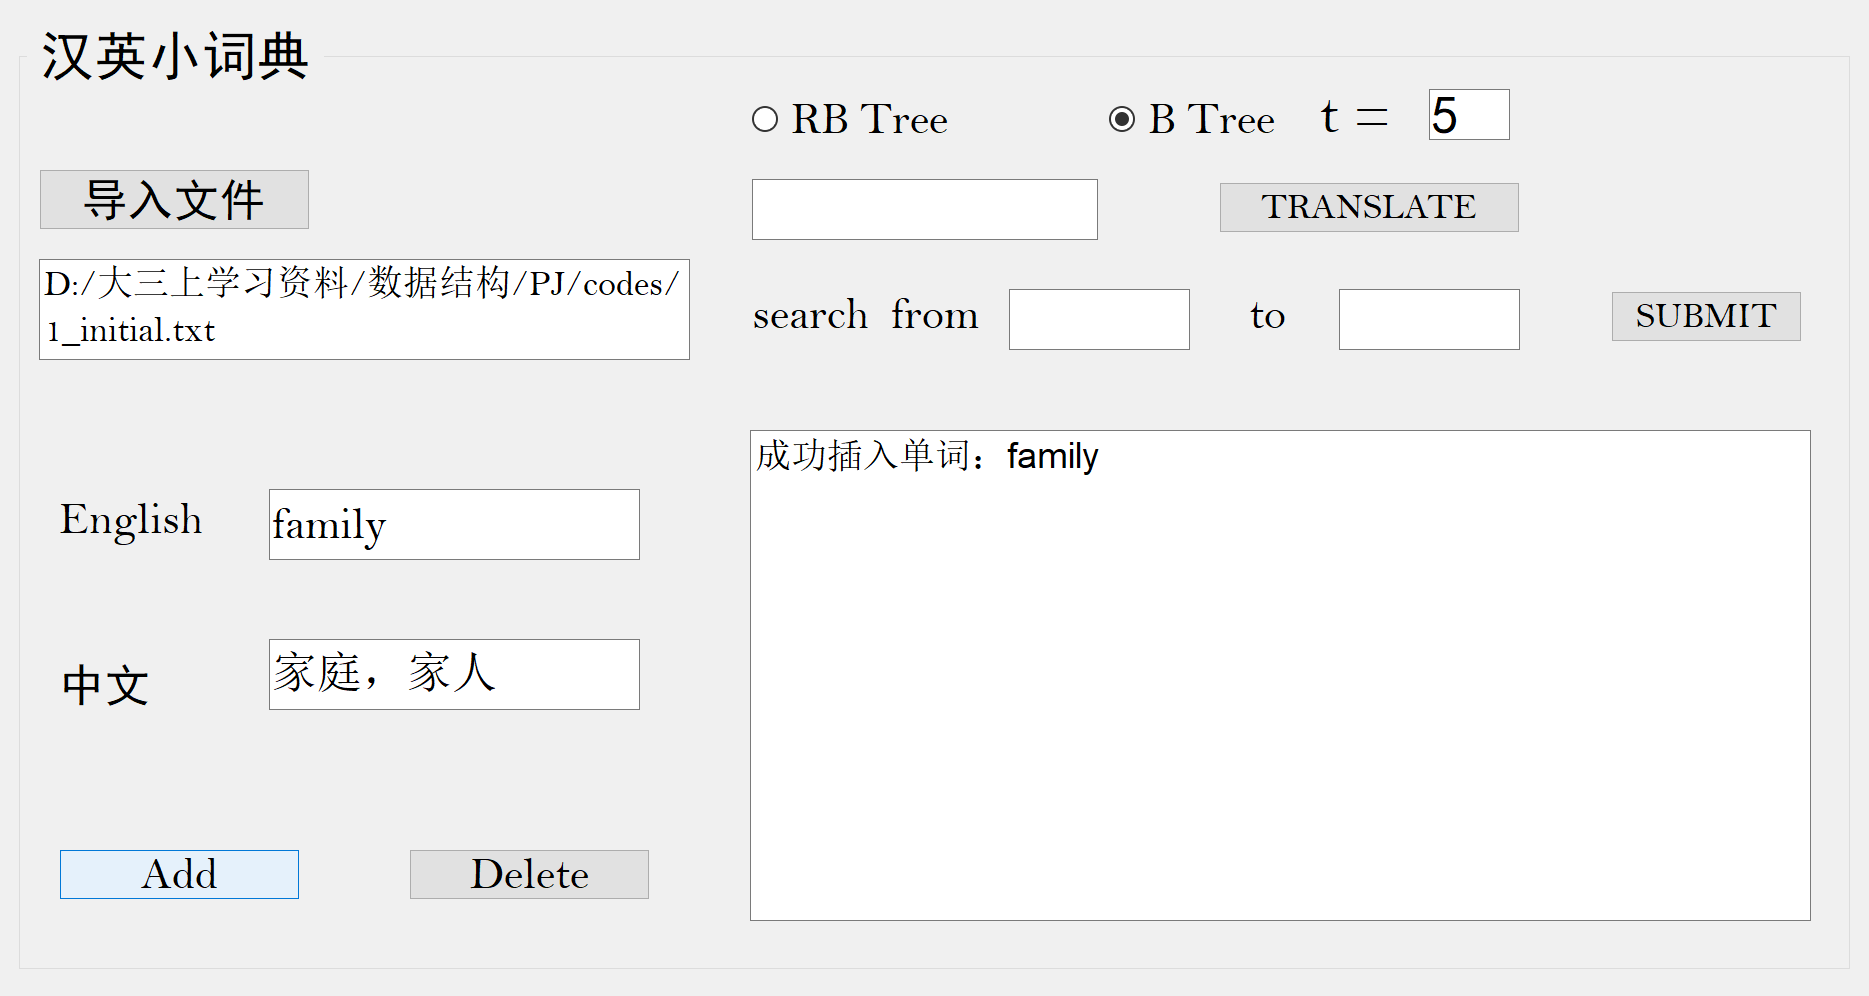
\includegraphics[width=0.45\textwidth]{GUI//第一次插入.png}}
    \,    
    \subfigure[无法插入一个已经存在的单词]
    {\label{add.sub.2}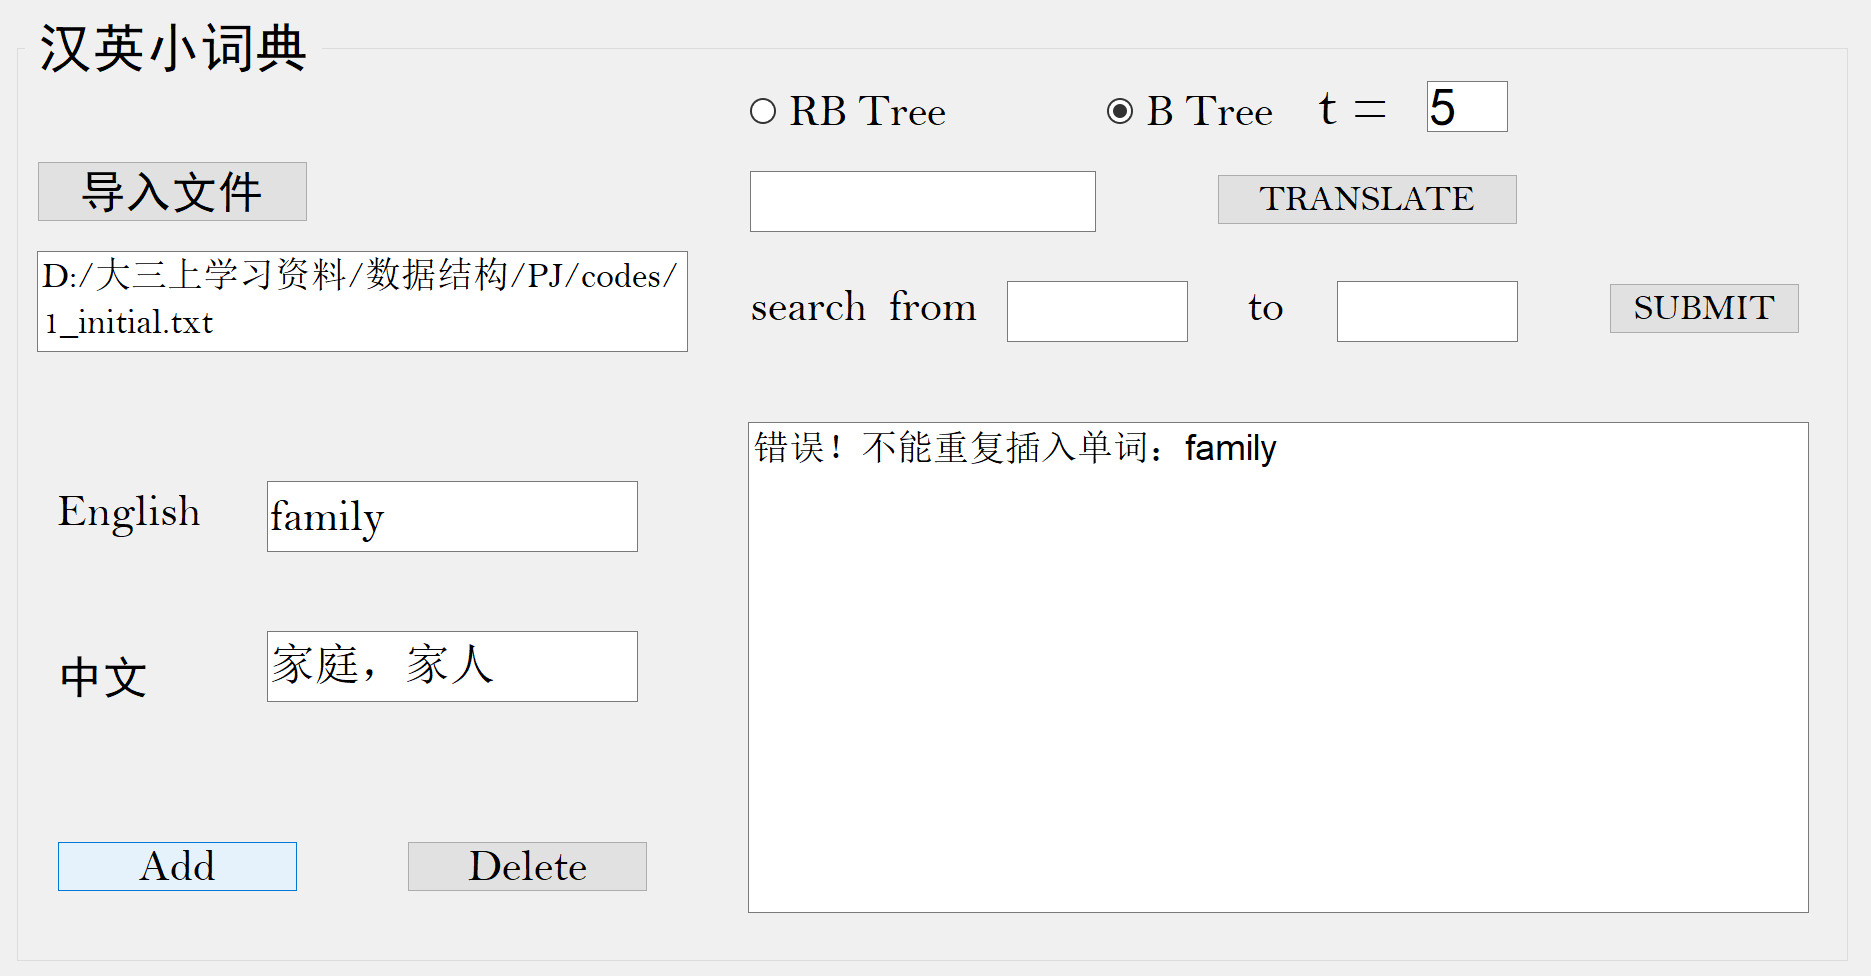
\includegraphics[width=0.45\textwidth]{GUI//重复插入.png}}
	\caption{插入单词}
	\label{add.main}
\end{figure}

\paragraph{删除单词} 点击左下方的"Delete"按钮,可以删除英文文本框中的对应单词。
如果词典中存在该单词,则可以成功删除,如图\ref{delete.sub.1}所示。如果不存在该单词,则无法删除,
并会抛出提示,如图\ref{delete.sub.2}所示。

\begin{figure}[H]
    \centering
    \subfigure[删除一个原本存在的单词] 
    {\label{delete.sub.1}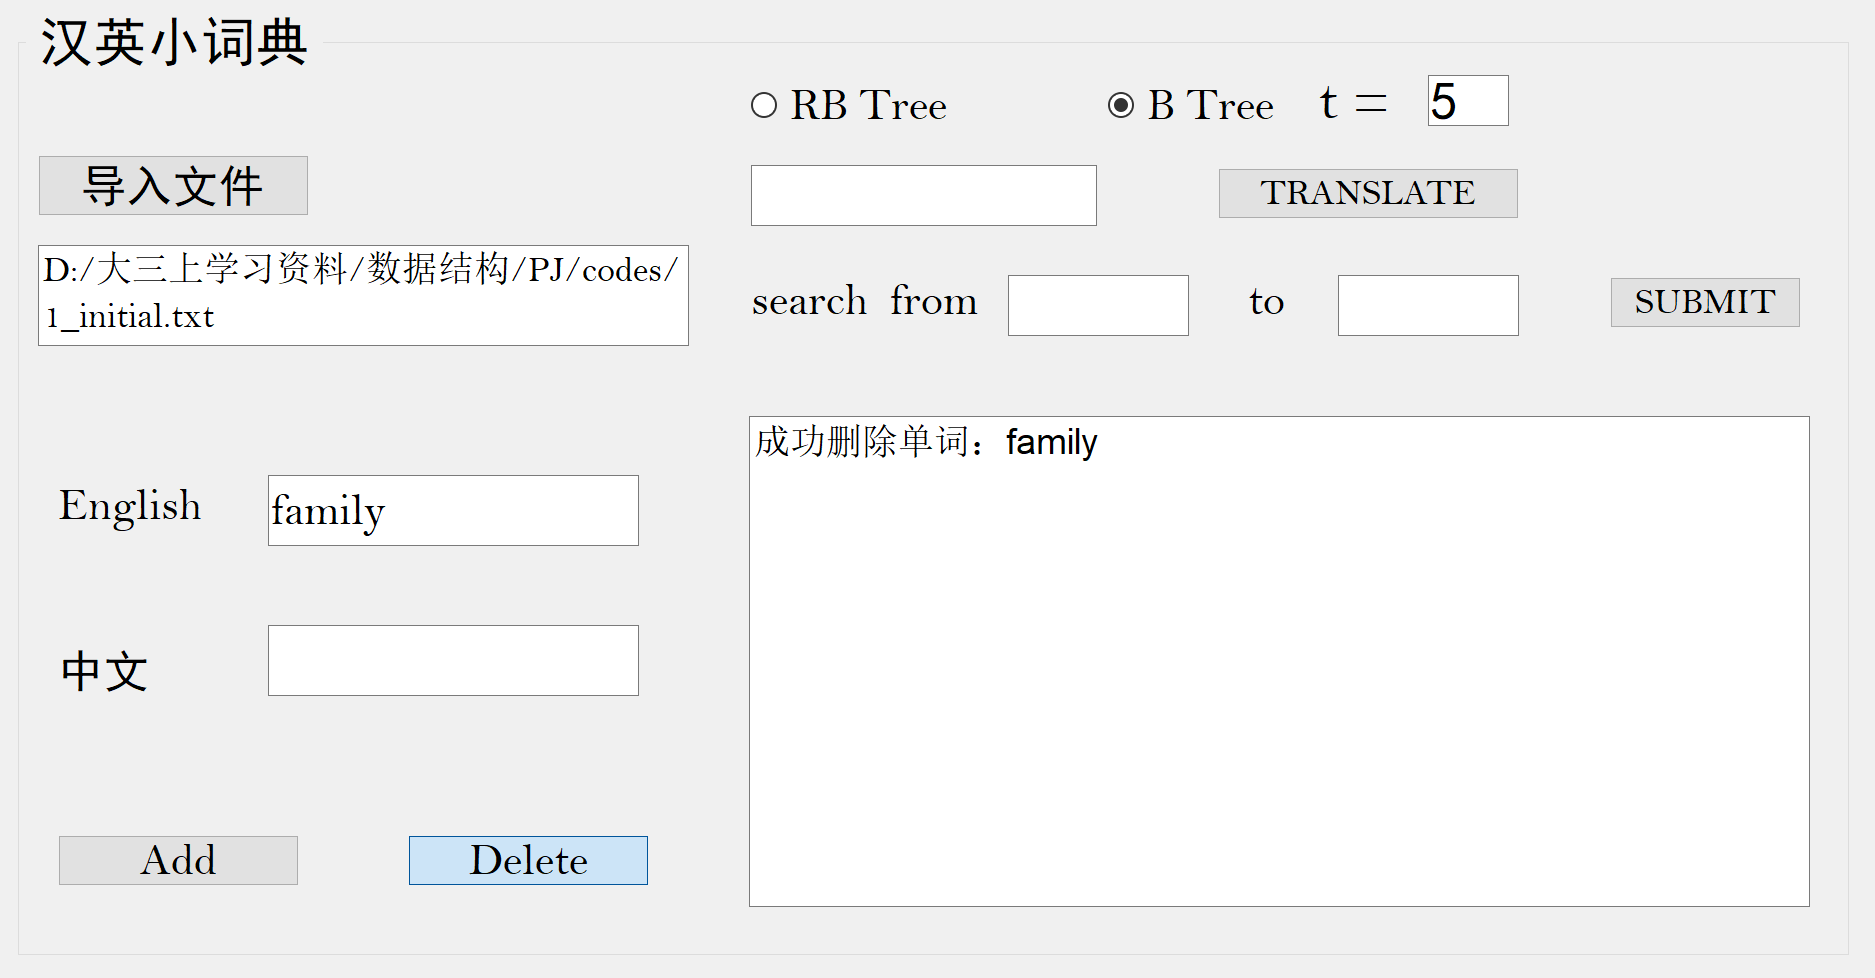
\includegraphics[width=0.45\textwidth]{GUI//第一次删除.png}}
    \,    
    \subfigure[删除一个不存在的单词]
    {\label{delete.sub.2} 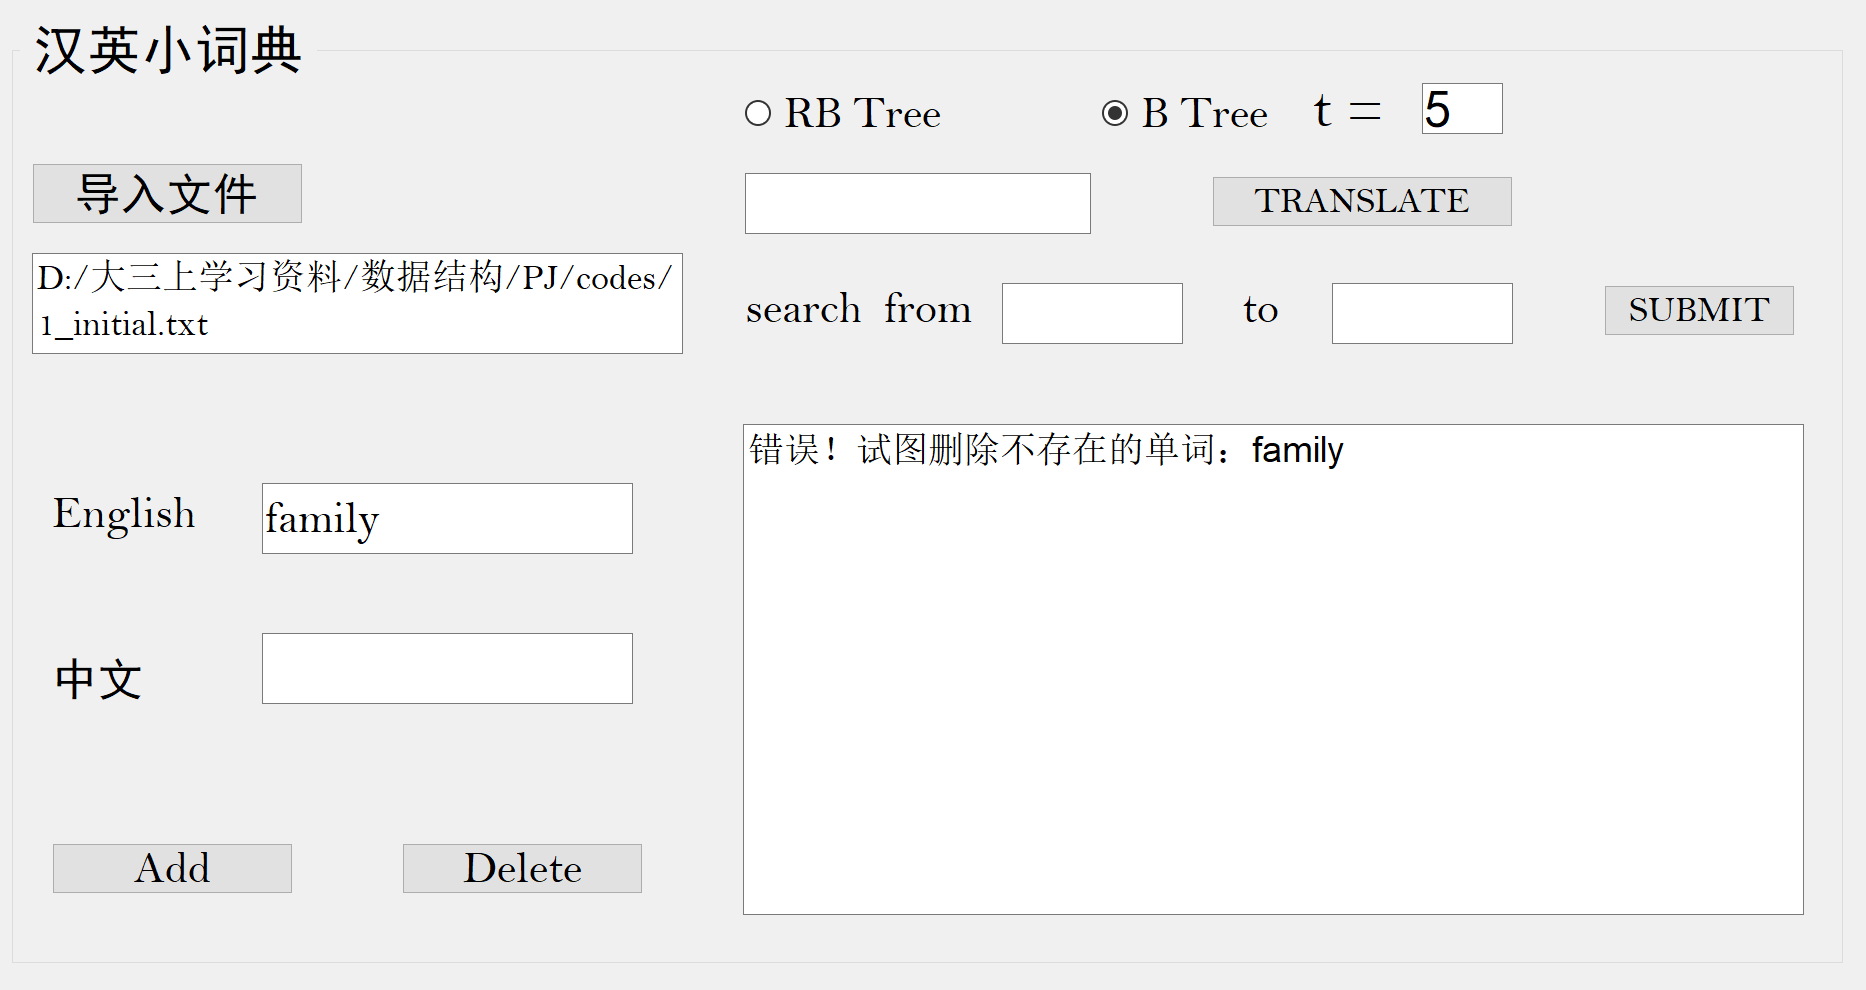
\includegraphics[width=0.45\textwidth]{GUI//重复删除.png}} 
	\caption{删除单词}
	\label{delete.main}
\end{figure}


\paragraph{查询单词} 界面右侧中部的按钮"Translate"提供单词查询功能。
如果所查的单词在词典中存在,则会返回单词的英文和中文,如图\ref{get.sub.1}所示。
如果所查的单词在词典中不存在,则会弹出错误提示,如图\ref{get.sub.2}所示。

\begin{figure}[H]
    \centering
    \subfigure[查询一个存在的单词] 
    {\label{get.sub.1}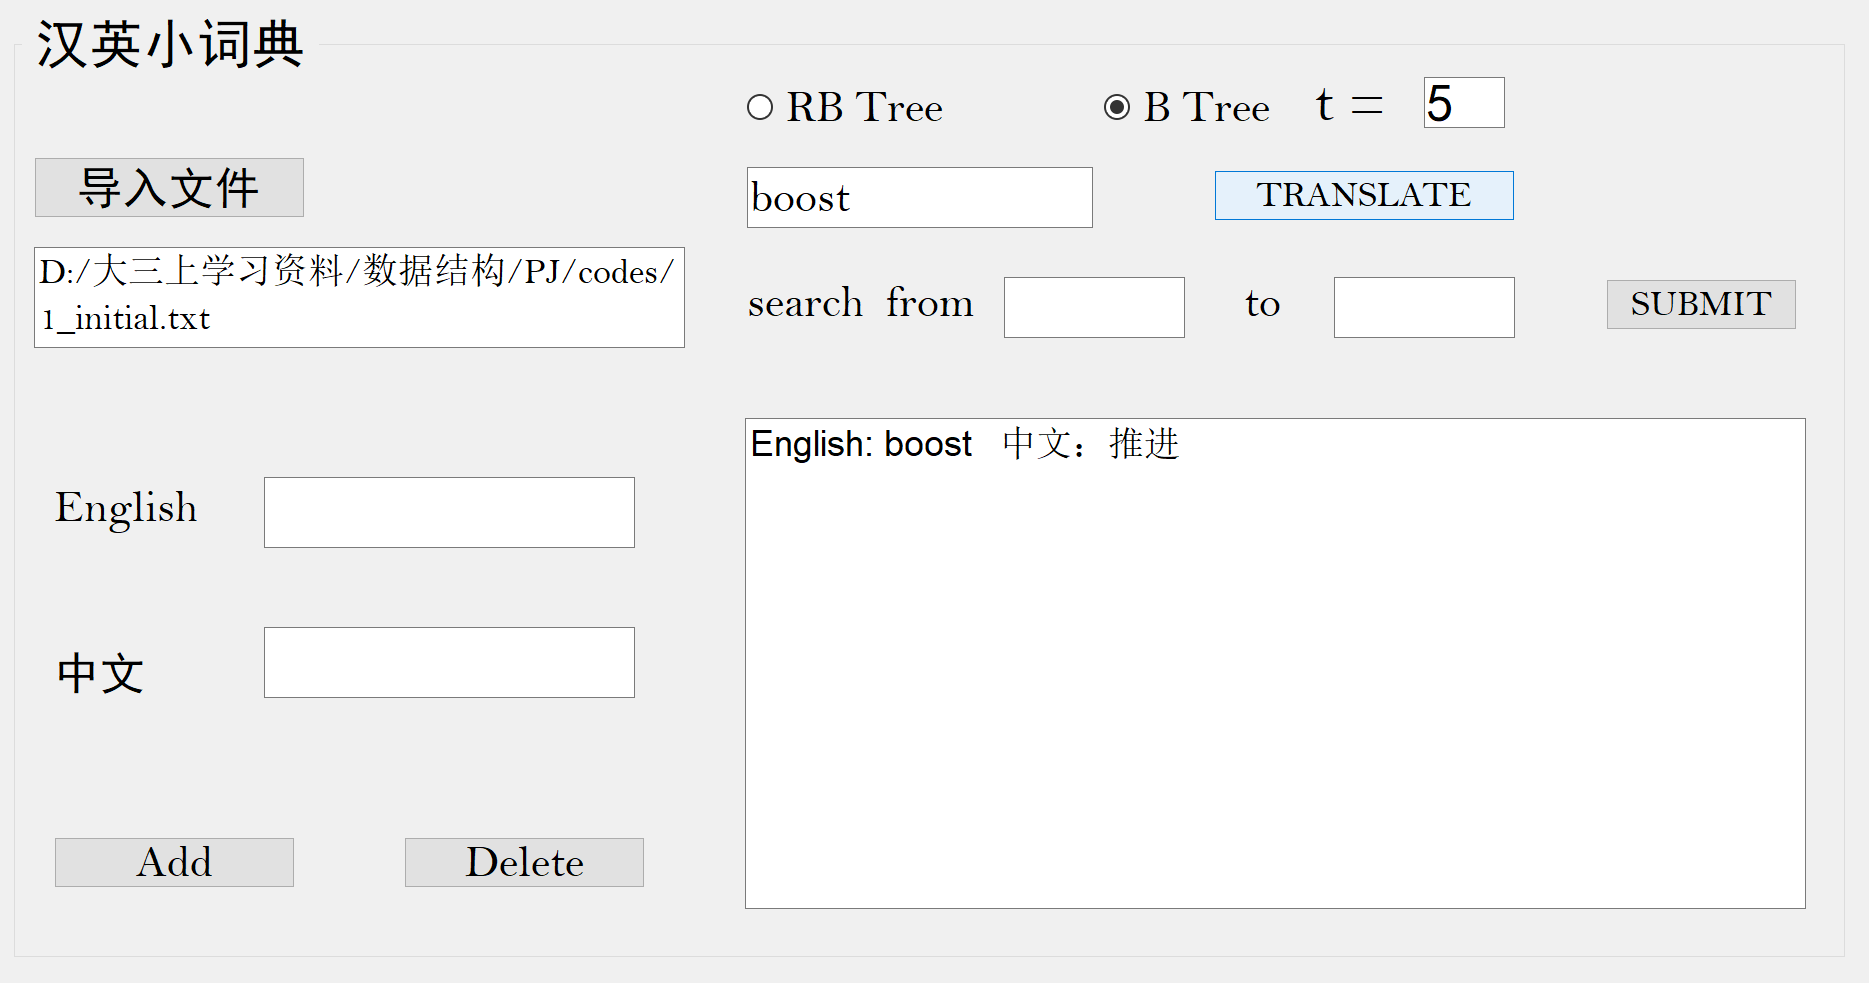
\includegraphics[width=0.45\textwidth]{GUI//查询存在单词.png}}
    \,    
    \subfigure[查询一个不存在的单词]
    {\label{get.sub.2}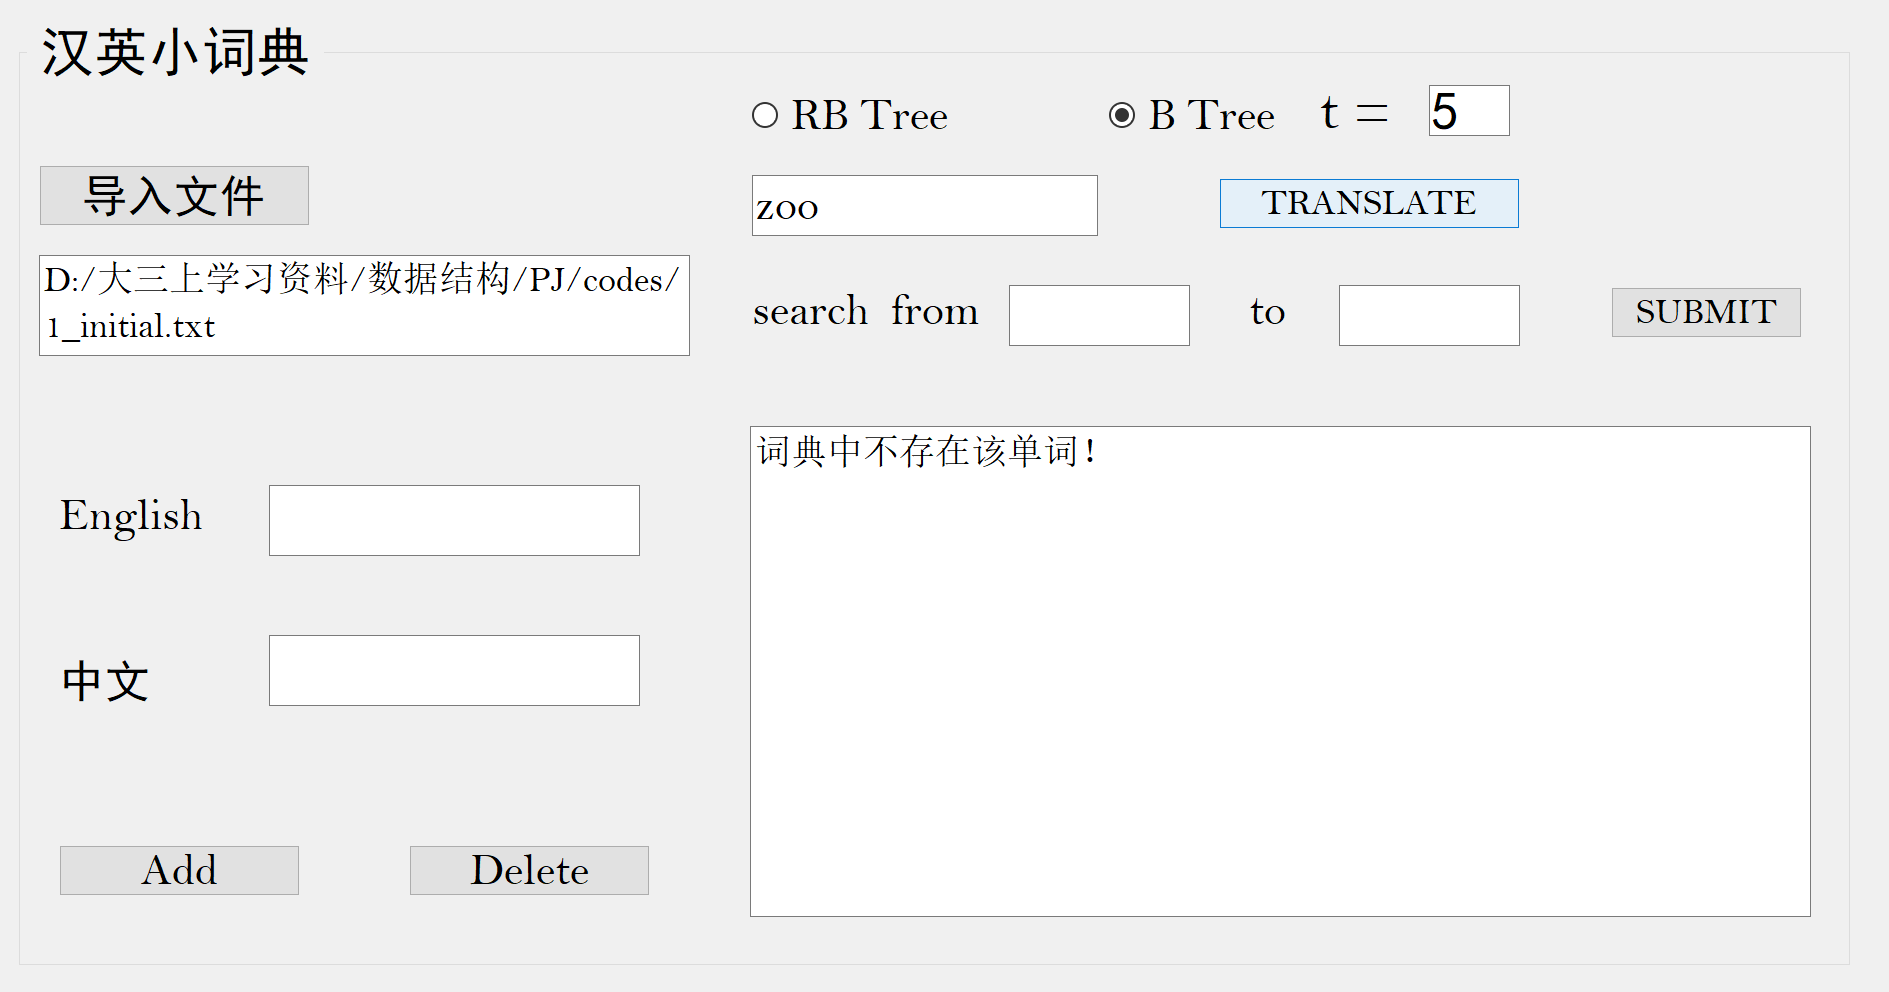
\includegraphics[width=0.45\textwidth]{GUI//查询不存在词.png}}
	\caption{查询单词}
	\label{get.main}
\end{figure}

\paragraph{按照给定范围查询单词}
在界面的右侧中部位置,还有一个"Submit"按钮,点击该按钮,可以查询在给定范围内的单词。
这里我们以"ac"到"acz"之间的单词为例进行查询,结果如下:
\begin{figure}[H]
	\centering
	{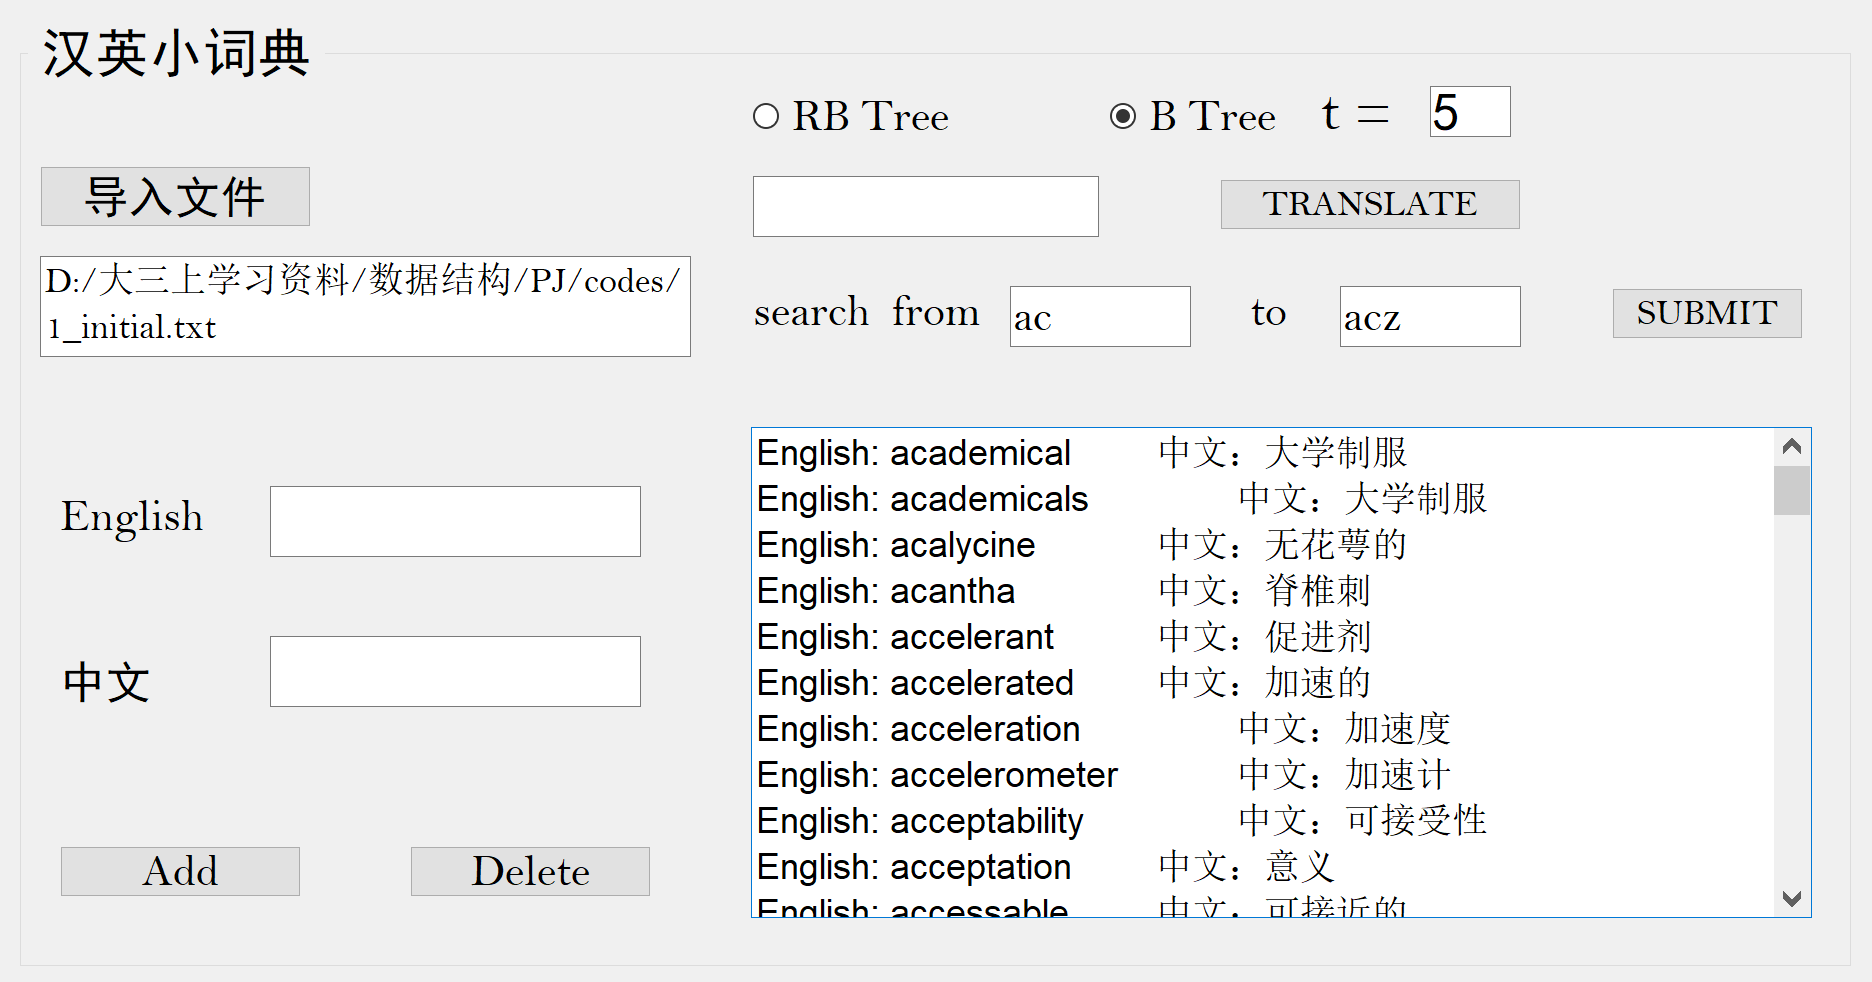
\includegraphics[width=0.5\textwidth]{GUI//范围查询.png}} 
	\caption{按照范围查询单词}
\end{figure}



\section{创新点:结合词典实际情况,重新设计单词排列顺序}
在Python默认的字符串比较运算中,比较是逐位基于字母的ASCII码进行的,由于大写字母的ASCII码都小于
小写字母的ASCII码,因此会出现"book" > "China"的现象,也即"China"排在"book"的前面;
但事实上我们希望的是"China"排列在"book"的后面。

因此,我利用Python的字典结构,重构了字符串的比较方式。在我设计的比较中,字母的顺序按照
\textbf{从小到大的顺序}依次为"AaBbCcDdEeFfGgHhIiJjKkLlMmNnOoPpQqRrSsTtUuVvWwXxYyZz",
这样就符合我们日常使用的英语词典的排列顺序了。

此外,对于起始部分相同的单词,我设定长的单词“大于”短的单词,例如对于单词"cat"和"catch",都以cat开头,
但由于"catch"单词更长,因此会排在"cat"的后面,这也是和日常使用的英语词典的排列方式是一致的。


\section{附录:B树的初始化耗时记录}

\paragraph{t=5} 
0.0, 0.003935813903808594, 0.003267526626586914, 0.003990888595581055, 0.0, 0.006471395492553711, 0.003665924072265625, 0.0039997100830078125, 0.0047607421875, 0.0010104179382324219, 0.003996610641479492, 0.006261348724365234, 0.0018956661224365234, 0.0039997100830078125, 0.004820585250854492, 0.003999948501586914, 0.004010438919067383, 0.0026171207427978516, 0.003999948501586914, 0.004010915756225586, 0.0049746036529541016, 0.003999948501586914, 0.004000425338745117, 0.004001140594482422, 0.004000663757324219, 0.003000974655151367, 0.0010187625885009766, 0.003999948501586914, 0.008002758026123047, 0.004066944122314453, 0.003943443298339844, 0.0, 0.004000663757324219

\paragraph{t=10}
0.002998828887939453, 0.0030007362365722656, 0.004029989242553711, 0.0024030208587646484, 0.0039997100830078125, 0.0067789554595947266, 0.004000186920166016, 0.0040013790130615234, 0.0050983428955078125, 0.004886627197265625, 0.0049381256103515625, 0.0039997100830078125, 0.005408525466918945, 0.005324840545654297, 0.0040013790130615234, 0.005789041519165039, 0.005001068115234375, 0.005001544952392578, 0.00400090217590332, 0.004239320755004883, 0.003999471664428711, 0.00401616096496582, 0.003997802734375, 0.0043888092041015625, 0.0076045989990234375, 0.004001140594482422, 0.00400090217590332, 0.00400090217590332, 0.008002281188964844, 0.005207061767578125, 0.006345510482788086, 0.003997087478637695, 0.004999637603759766

\paragraph{t=15}
0.006587028503417969, 0.003929615020751953, 0.0045375823974609375, 0.002009153366088867, 0.007999897003173828, 0.005751132965087891, 0.0074841976165771484, 0.0038199424743652344, 0.008864879608154297, 0.004000425338745117, 0.006421566009521484, 0.008001089096069336, 0.0034368038177490234, 0.008907556533813477, 0.0043790340423583984, 0.007703065872192383, 0.0060002803802490234, 0.006341218948364258, 0.007999420166015625, 0.0030362606048583984, 0.008965730667114258, 0.005930423736572266, 0.0061779022216796875, 0.004000425338745117, 0.007723331451416016, 0.00800180435180664, 0.004879951477050781, 0.007718324661254883, 0.00700068473815918, 0.008002519607543945, 0.007000446319580078, 0.005948066711425781, 0.00789952278137207


\paragraph{t=20}
0.004000663757324219, 0.004000425338745117, 0.0050013065338134766, 0.0050013065338134766, 0.006000518798828125, 0.007001638412475586, 0.008002519607543945, 0.008002042770385742, 0.007001161575317383, 0.0060007572174072266, 0.009003162384033203, 0.007000446319580078, 0.007003068923950195, 0.007000923156738281, 0.0060007572174072266, 0.007002353668212891, 0.007002353668212891, 0.006000518798828125, 0.007000923156738281, 0.007002353668212891, 0.006002187728881836, 0.007000923156738281, 0.007001161575317383, 0.008002758026123047, 0.007001161575317383, 0.0070035457611083984, 0.009002208709716797, 0.010001420974731445, 0.007002353668212891, 0.008001565933227539, 0.009001970291137695, 0.008002042770385742, 0.007001399993896484


\paragraph{t=25}
0.004000425338745117, 0.005002021789550781, 0.00500035285949707, 0.006002902984619141, 0.005999565124511719, 0.0070018768310546875, 0.009001970291137695, 0.007001638412475586, 0.00800180435180664, 0.008001327514648438, 0.008002758026123047, 0.008000850677490234, 0.008002281188964844, 0.006001472473144531, 0.008001565933227539, 0.007001399993896484, 0.00800180435180664, 0.009002685546875, 0.009001731872558594, 0.007001399993896484, 0.007001638412475586, 0.009002447128295898, 0.008001565933227539, 0.008001327514648438, 0.010002613067626953, 0.007001399993896484, 0.009002208709716797, 0.008002042770385742, 0.009001970291137695, 0.010002613067626953, 0.010001420974731445, 0.010002851486206055, 0.008001565933227539


\end{document}

% \begin{figure}[H]
% 	\centering
% 	{\includegraphics[width=0.35\textwidth]{image//ignorance.png}} 
% 	\caption{}
% \end{figure}


% \lstinputlisting[style = Python,
% caption={Python codes},
% label = {efficient},
% linerange={110-125}]{exercise3.py} 


% \begin{figure}[H]
%     \centering
%     \subfigure[patch size = 11]
%     {\includegraphics[width=0.49\textwidth]{image//local equalization with patch size = 11.jpg}}
%     \,    
%     \subfigure[patch size = 51]
%     {\includegraphics[width=0.49\textwidth]{image//local equalization with patch size = 51.jpg}}
%     \,
%     \subfigure[patch size = 151]
%     {\includegraphics[width=0.49\textwidth]{image//local equalization with patch size = 151.jpg}}
%     \,    
%     \subfigure[patch size = 201]
%     {\includegraphics[width=0.49\textwidth]{image//local equalization with patch size = 201.jpg}}
%     \caption{local equalization with different patch sizes}
% \end{figure}
